% !TeX root =thesis.tex



\newcommand{\htd}{\tilde{h}}
\chapter{The two-channel three-species many-body model, the mean field\label{ch:path2}}


For the narrow Feshbach resonance, atoms have considerable weight in the closed-channel and the Pauli exclusion between two channels cannot be neglected.  A many-body framework needs to include both channels.  Before diving into the detailed calculation, let us make some rough estimates about scales in order to  build some intuition.  The same problem at the two-body level is well understood as briefed in Chapter \ref{sec:intro:twobody}.  %Extended to many-body, three different types of Pauli exclusion requires to be considered: Pauli exclusion within open-channel, Pauli exclusion within closed-channel and Pauli exclusion between two channels. Let us estimate the scale of each with an artificial question.  We  calculate how much is reduced in two-body wave function by one single type of Pauli exclusion when a new pair is added.  This quality is quite unphysical without any real measurable counterpart, but it serves as a starting point to build intuition. 
We estimate how much each channel would change  in a many-body system.  Compared to a two-body system, the two-body correlation in a (cold) many-body fermion system is modified mostly in  low  energy,  around or below the Fermi energy, while staying  just like  the two-body wave-function intact in high energy.  The open-channel component  of the two-body scattering wave-function is like a zero-energy free wave ($k=0$) plus a small kernel of size $r_c$.  In momentum space, this wave function is like a $\delta$-function at $k=0$ with a small tail.  The occupation number in the first available level, $k=0$, is close to one (for two hyperfine spins) and this level cannot accommodate one more pair.  The next pair has to occupy the next available level in $k$ instead of the lowest energy two-body level, $k=0$.  This suggests that the open-channel requires a full many-body treatment.  The situation is quite different in the closed-channel.   One crucial assumption is that  the closed-channel bound state is much smaller than the interparticle distance. A closed-channel bound state,  $\phi_{0}$, spreads its most weight  in the  momentum range $[0,1/a_{c}]$.  The weight in each momentum level is so tiny that it is even smaller than $1$ when it is multiplied by total atoms number $N$, $N\abs{\phi_{k}}^{2}\ll1$.             It only has a very small fraction of its weight within the Fermi energy range ($<k_{F}$).  Hence, the closed-channel only has a small possible overlap with atoms in  the open-channel, as well as with other atoms in the closed-channel.  The smallness of this overlap ensures that many-body effects in the closed-channel can be  treated perturbatively.  As discussed in Sec. \ref{sec:intro:as} and Appendix \ref{sec:pathInt2:short-range}, the high momentum part of the two-body correlation just follows the two-body wave function;  therefore, we can write two-body correlation as 
\begin{equation}\label{eq:pathInt2:hphif}
h_{\vk}\sim\phi_{0\vk}f(\vk)
\end{equation}
 with $f(\vk)=1$ for $k\gg{k_{F}}$.  $f(\vk)$ deviates from $1$ in low energy and represents all the many-body correction. 

%This is fairly straight-forward Pauli exclusion within open-channel.  Open-channel wave function is almost like a free wave ($k=0$) with small kernel in $r_c$.  The open-channel is like a Fermi sea with clear step at chemical potential in BCS side. It is less step-like in BEC  side, nevertheless, the lowest level ($k=0$) occupation is large and in the order $1$.   If adding a pair with the original wave-function, the normalization is simply going to be reduced by a factor in order of $1$.  Actually in BCS side, the next open-channel pair can only occupy the next $k$ level, which is nothing like the two-body wave function at all.  A many-body state is nothing like the simple exponential of two-body wave function.  Therefore, this type of Pauli exclusion calls for the most exact treatment, and indeed, we takes the anomalous correlation function, gap, and carry the non-perturbative (BCS) treatment all the way.
%
% Pauli exclusion within closed-channel is just the opposite.  Given the assumption that the size of closed-channel bound state, $a_c$, is much smaller than the average particle distance, $a_0$.  ????  This effect is in the order of $(a_c/a_0)^4$ (\cite{CobosonPhysicsReports}). ??????    We are going to ignore this effect most of time by taking close-close two-body correlation simply as two-body wave-function $\phi_0$ at high-momentum.  
% 
% The inter-channel Pauli exclusion sits in between of them.  If we take the open-channel as a simple Fermi gas (liquid).  The wave function of closed-channel bound state $\phi_0$ spreads over $[0,1/a_c]$ in momentum space, a simple estimation of the overlap with open-channel Fermi sea is  $k_F^3(1/a_c)^{-3}\sim(a_c/a_0)^3\ll1$.  This effect is larger than the Pauli exclusion within closed-channel but smaller than 1, therefore, we handle it perturbatively.  
%
In addition, the model needs to be explicitly expressed with the three hyperfine species in order to address the Pauli exclusion between two channels due to the common species.  This effect has received little  attention in theoretical research and a model as such is a useful addition to our knowledge of the BEC-BCS crossover and the Feshbach resonance.  On the other hand, as we just discussed, and will illustrate more quantitatively later, the effects of the inter-channel Pauli exclusion in the closed-channel is relatively minor and can be treated perturbatively.  Consequently, it is not necessarily to carry the three species description all through the calculation as in a genuine three species fermion problem.  Description of two channels and description of three species are used in different phases of the calculation to solve the problem.  

\section{The extremely narrow resonance\label{sec:pathInt2:extremelyNR}}
Before the quantitative model, we discuss qualitatively a simple yet revealing case,   the extremely narrow resonance, where the inter-channel coupling approaches zero, $Y\rightarrow0$.  In this case, two channels are almost independent to each other except sharing the same chemical potentials.  From the two-body discussion in Chapter \ref{sec:intro:twobody} (Eqs. \ref{eq:intro:Krr}, \ref{eq:intro:kappa}, \ref{eq:intro:deltaC}), the characteristic width of the resonance $\delta_{c}$ is zero in this case, which indicates that the resonance is always narrow no matter how dilute the system is.  


\begin{figure}[hhtb]
	\centering
	         \subfloat[$E_{F}<\tilde\delta$]{\label{fig:narrowFR:aboveSea}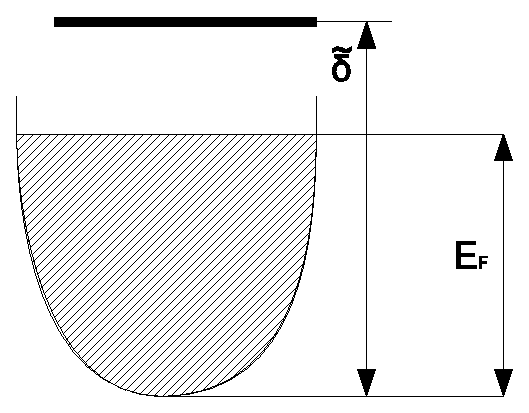
\includegraphics[width=.2\textwidth]{narrowFRabove.eps}}\quad
		\subfloat[$0<\tilde\delta<E_{F}$]{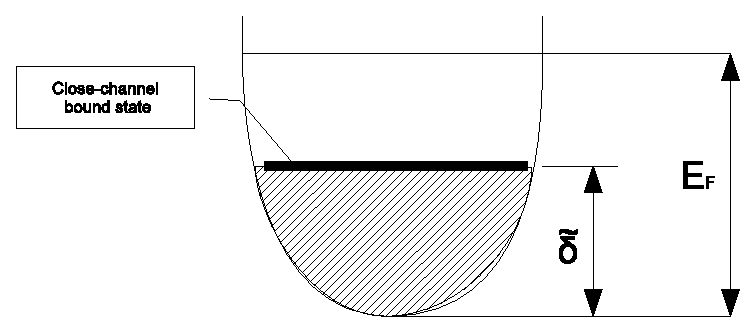
\includegraphics[width=.30\textwidth]{narrowFRin.eps}\label{fig:narrowFR:inSea}}\quad
		\subfloat[$\tilde\delta<0$]{\label{fig:narrowFR:belowSea}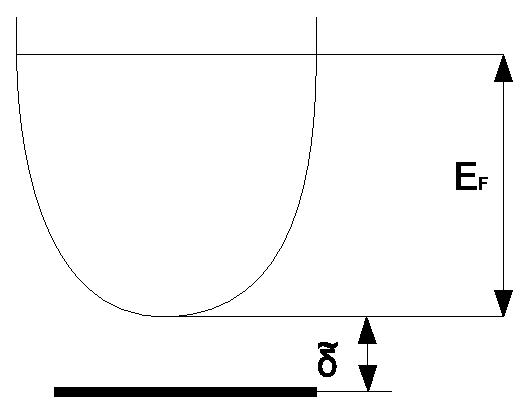
\includegraphics[width=.20\textwidth]{narrowFRbelow.eps}}
	\caption{Extremely narrow resonance\label{fig:narrowFR}}
	\small{The shaded area is occupied by atoms. }
	%\parbox{0.7\textwidth}{\small{  In Fig. \subref{fig:narrowFR:inSea} chemical potential would be close to the closed-channel bound state level (besides small shift due to the open-channel intra-channel coupling) and the ``Fermi sea'' above is empty. }}
\end{figure}
Here we assume that the atoms in the open-channel maintains a relatively clear Fermi surface, like the Fermi liquid or the BCS.  The many body situation is  quite straightforward. In general, three different situations exist, as Figs. \ref{fig:narrowFR:aboveSea}, \ref{fig:narrowFR:inSea} and \ref{fig:narrowFR:belowSea}.  When the closed-channel bound state level is above the Fermi sea ($E_{F}<\tilde\delta$, Fig. \ref{fig:narrowFR:aboveSea}), all atoms are in the open-channel and no atoms in the closed-channel.  Therefore, it is a genuine  single-channel problem (only open-channel) with the original bare open-channel interaction.   There is no need to considering the inter-channel Pauli exclusion.  When the closed-channel bound state level is below the Fermi sea ($\tilde\delta<0$, Fig. \ref{fig:narrowFR:belowSea}), all atoms are in the closed-channel and no atoms in the open-channel.  It is a simple di-atom molecule gas. There is no need to considering the inter-channel Pauli exclusion either.  The interesting situation is when the closed-channel bound state is in the Fermi sea  ($0<\tilde\delta<E_{F}$, Fig. \ref{fig:narrowFR:inSea}).  The Fermi sea is then filled from the bottom (zero energy) all the way to the closed-channel bound state level in the open-channel.  Then all the rest atoms go into the closed-channel.  We do need to consider the inter-channel Pauli exclusion because atoms exist in both channel.  




We can image the two channels are decoupled and each has $N^{(o)}$ ($N^{(c)}$ atoms.  It is not hard to find the wave function in each case.  The inter-channel Pauli-exclusion effect should be in the order of the overlap of these two wave functions. In the open-channel, the momentum space is filled  with occupation $1$ from the bottom up to the order $E_F$ (or $\tilde\delta$). In the closed-channel, as we discussed in the introduction, the occupation is roughly $1/E_b$ at the low momentum ($\lesssim{}E_F$), where $E_b$ is the binding energy of the closed-channel bound state.   So this effect should be roughly is equal $E_F/{E_b}$.

\section{Model set-up and the Hubbard-Stratonovich transformation}

One way to approach this problem is to extend BCS ansatz and then find the set of parameters that optimizes the free energy.  We can write down a  three species BCS ansatz as 
\begin{equation}\label{eq:pathInt2:ansatz}
\ket{\Psi}=\prod_\vk\br{u_\vk+v_\vk{}a^\dg_\vk{}b^\dg_{-\vk}+w_\vk{}a^\dg_\vk{}c^\dg_{-\vk}}\ket{0}
\end{equation} 
with normalization, $\abs{u_\vk}^2+\abs{v_\vk}^2+\abs{w_\vk}^2=1$.   Here ``$a$'' is the common species of two channels. $(a,b)$ is the open channel and $(a,c)$ is the closed channel.  $\ket{0}$ is the vacuum state of fermions. This ansatz can be derived from a many-body coherent state of the two-body state as we did in the single-channel (Eq. \ref{eq:intro:BCScoherent}), 
\begin{equation}\label{eq:pathInt2:ansatzCoh}
\ket{\Psi}\propto\exp{}\mbr{\sum_{\vk}(\phi^{(ab)}_\vk{}a^\dg_\vk{}b^\dg_{-\vk}+\phi^{(ac)}_\vk{}a^\dg_\vk{}c^\dg_{-\vk})}\ket{0}
\end{equation} 
$\phi^{(ab)}$ and $\phi^{(ac)}$ are related to $u_\vk$, $v_\vk$ and $w_\vk$ as  
\begin{gather}
\phi_{\vk}^{(ab)}=\frac{v_{\vk}}{u_{\vk}}\\
\phi_{\vk}^{(ac)}=\frac{w_{\vk}}{u_{\vk}}\label{eq:pathInt2:phiWU}
\end{gather}
 We can then proceed to find the set of $(u_{\vk},v_{\vk},w_{\vk})$ that optimizes the free energy. This method offers good intuition of the state  with an explicit connection to the two-body wave function, $\phi^{(ab)}$ and $\phi^{(ac)}$, .  However,  it is not easy to find these parameters from optimization process. Furthermore, it is hard to extend this method beyond the mean-field to study phenomena such as collective modes.  We briefly discuss this approach in Appendix \ref{ch:mean}. Instead, in this chapter, we use the path integral method, which turns out to be  more convenient for our problem.   The Hubbard-Stratonovich transformation provides a powerful tool for studying non-trivial degrees of freedom (order parameters) in the system.  It is more or less equivalent to other approaches at mean-filed level. But it has great advantage to be easily extended to explore the fluctuation over the mean-field result.  

For a two-channel problem, we write down the Hamiltonian \footnote{Here and hereafter in the chapter, we take $\hbar=1$.} as
\begin{equation}\label{eq:pathInt2:ham2}
\begin{split}
H&=\int{d^{d}r}\bigg\{\sum_{j=(a,b,c)}\bar\psi_{j}\mbr{\nth{2m}(-i\nabla)^{2}-\mu+\eta_{j}}\psi_{j}\\
	&\qquad-U\bar\psi_{a}(r)\bar\psi_{b}(r)\psi_{b}(r)\psi_{a}(r)-V\bar\psi_{a}(r)\bar\psi_{c}(r)\psi_{c}(r)\psi_{a}(r)\\
	&\qquad-\mbr{Y\bar\psi_{a}(r)\bar\psi_{b}(r)\psi_{c}(r)\psi_{a}(r)+h.c.}
	\bigg\}
\end{split}
\end{equation}
Here $\eta_{j}$ is the Zeeman energy of the specific hyperfine species.  $a,b,c$ stands for the three hyperfine species defined as the same before in the ansatz approach.  All the interactions ($U$, $V$, $Y$), are contact type, this simplifies the Hubbard-Stratonovich transformation considerably.  It is plausible as we only study low-energy phenomena for the short-range potential. 

A contact interaction is  flat in momentum space, in other words, it pairs not only zero center-of-mass momentum pairs, but also finite center-of-mass momentum pairs, unlike the paring interaction used in the original BCS work\cite{BCS}, which only pairs zero center-of-mass momentum, i.e. opposite-momentum, pairs.  Nevertheless, the saddle point (mean-field) solution settles at the zero center-of-mass momentum pairing; therefore the mean-field solution coincides with that of  variation method derived from pairing  only opposite momentum atoms.  On the other hand, the collective mode (fluctuation of order parameters) emerges naturally from the included non-zero center-of-mass momentum interaction.  We do not need to introduce more general interaction terms beyond the simple opposite momentum pairing (e.g. the Coulomb interaction in \cite{AndersonBCS}) to study collective modes.   

Three different types of Hilbert spaces are used in this chapter.   The first one is the  (infinite dimension) coordinate space and its reciprocal momentum space.   The second one is the  (3 dimension) space of hyperfine spin, $a,\,b,\,c$.   These two are atom-based.  The full many-body Hilbert space is $N$-power (also direct-product type) of the direct product of these two.  As discussed previously, in some cases, instead of a 3-dimension hyperfine space, we use the third type of spaces, open- and closed-channel, $(a,b),\,(a,c)$ (2 dimension).  Strictly speaking, this one is just a subspace of the direct product of a pair hyperfine spin spaces.  Nevertheless,  it is sufficient within our model because only these two combinations (channels) of a pair are considered.    In principle, fermion fields $\psi$ and $\bar\psi$ (and $\Delta$ and $\bar\Delta$ defined according to $\psi$ and $\bar\psi$),  both Grassmann numbers, are independent to each other  and  not related as complex conjugate\footnote{Complex conjugate is not a well-defined concept for Grassmann algebra}.  This is marked by using ``$\bar{\;}$''(bar) instead of the normally used ``$^{\dg}$''(dagger) sign. In this chapter, a $3\times3$ matrix always refer to hyperfine spins; while a $2\times2$ matrix always refers to  open- and closed-channel.  And $^{}\dg$ sign  is reserved only for hermitian conjugate of these two types of matrices. 
%We can introduce a unitary transformation $Q$ (mixing two channels) to diagonalize the interaction matrix into diagonal matrix $A$.
%\begin{equation}
%\begin{split}
%Q^{\dg}AQ=\mtrx{U&Y\\Y^{*}&V}\equiv{}\tilde{U}\\
%\tilde{U}\equiv\mtrx{U&Y\\Y^{*}&V}=Q\mtrx{A_{11}&0\\0&A_{22}}Q^{\dg}
%\end{split}
%\end{equation}

Introduce two channels into the vector form.    $(\psi\psi)$  is a column vector and $(\bar\psi\bar\psi)$ is a row vector.
\begin{equation*}
(\bar\psi\bar\psi)=\mtrx{\bar\psi_{a}\bar\psi_{b}&\bar\psi_{a}\bar\psi_{c}}
\qquad(\psi\psi)=\mtrx{\psi_{b}\psi_{a}\\\psi_{c}\psi_{a}}
\end{equation*}
The two-body interaction can then be written as a ($2\times2$)  hermitian  matrix  $\tilde{U}$ in the channel space
\begin{equation}
\tilde{U}\equiv{}\mtrx{U&Y\\Y^{*}&V}
\end{equation}
We can now write the Hamiltonian in a more compact form
\begin{equation}
H=\int{d^{d}r}\bigg\{\sum_{j={a,b,c}}\bar\psi_{j}\mbr{\nth{2m}(-i\nabla)^{2}-\mu+\eta_{j}}\psi_{j}
 	-(\bar\psi\bar\psi)\tilde{U}(\psi\psi)
\end{equation}
The finite-temperature action is 
\begin{equation}\label{eq:pathInt2:actionFermi}
S(\bar\psi,\psi)=\int^{\beta}_{0}d\tau\int{d^{d}r}\mbr{\sum_{j}\bar\psi_{j}(\partial_\tau-\nth{2m}\nabla^{2}-\mu+\eta_{j})\psi_{j}
-(\bar\psi\bar\psi)\tilde{U}(\psi\psi)}
\end{equation}



Similar as in Chapter \ref{sec:pathInt}, we can perform the Hubbard-Stratonovich transformation on the action.   Introduce bosonic fields (functional variables), $(\Delta_{1},\Delta_{2})$, as a 2-component vector   and start from the ``fat identity'', where  all the integral constant is absorbed into the measure of functional integral of $\bigD(\Delta,\bar\Delta)$ \cite{Altland}.
\begin{equation}\label{eq:pathInt2:identity}
1=\int{\bigD(\Delta,\bar\Delta)}\exp(-\int{dx}\Delta^{\dg}\tilde{U}^{-1}\Delta)
\end{equation}
\[
\Delta^{\dg}=(\bar\Delta_{1},\bar\Delta_{2})\qquad\Delta=\begin{pmatrix}\Delta_{1}\\\Delta_{2}\end{pmatrix}
\]
here $x$ is four-coordinate, $(\vr, \tau)$,  $\int{dx}=\int^{\beta}_{0}d\tau\int{d^{d}\vr}$. 

We can make a shift in $\Delta$
\begin{equation}\label{eq:pathInt2:DeltaPhi}
\Delta\longrightarrow\Delta-\tilde{U}(\psi\psi)
\end{equation}
Write it explicitly into the matrix form
\begin{equation*}
\mtrx{\Delta_{1}\\\Delta_{2}}\longrightarrow
	\mtrx{\Delta_{1}\\\Delta_{2}}-
	\mtrx{U&Y\\Y^{*}&V}
	\mtrx{\psi_{b}\psi_{a}\\\psi_{c}\psi_{a}}
\end{equation*}
\begin{equation*}
\mtrx{\bar\Delta_{1},\bar\Delta_{2}}\longrightarrow
	\mtrx{\bar\Delta_{1},\bar\Delta_{2}}-
	\mtrx{\bar\psi_{a}\bar\psi_{b}&\bar\psi_{a}\bar\psi_{c}}
	\mtrx{U&Y^{*}\\Y^{}&V}
\end{equation*}
First of all, notice that the new auxiliary field $\Delta$ is related to the mixture of two channels by a $2\times2$ matrix $\tilde{U}$.
Also note that  $\bar{\Delta}_{i}$ is not the complex conjugate of $\Delta_{i}$ in general as they are related to Grassmann fields $\psi\psi$ and $\bar\psi\bar\psi$ which are not complex conjugate to each other. But it can be verified later that, to the  mean-field (saddle point) level as well as to the simple  (phase-fluctuation) Gaussian level about collective modes, $\bar{\Delta}_{i}$ and ${\Delta}_{i}$ are indeed complex conjugate (and real for saddle point).  Hence, for the simplicity, we will treat them as such hereinafter and use $\bar\Delta$ and $\Delta^{*}$ more or less arbitrarily.  The other point to notice is that, $\Delta(\vr,\tau)$ carries the the same coordinates as $\psi(\vr,\tau)\psi(\vr,\tau)$ (or frequency-momentum coordinates in the reciprocal space) because there is only the contact interaction.  Now the ``fat identity'' Eq. \ref{eq:pathInt2:identity} becomes 
\begin{equation}
1=\int{\bigD(\Delta_{j},\bar\Delta_{j})}\exp\big\{-\int{dx}
	[\Delta^{\dg}\tilde{U}^{-1}\Delta-(\bar\psi\bar\psi)\Delta-\bar\Delta(\psi\psi)+(\bar\psi\bar\psi)\tilde{U}(\psi\psi)]\big\}
\end{equation}
The above equation use the fact $\tilde{U}$ is hermitian, so $\tilde{U}^{\dg}\tilde{U}^{-1}=\tilde{U}^{-1}\tilde{U}=I$.
It can be rearranged as 
\begin{equation}
\exp[\int{dx}(\bar\psi\bar\psi)\tilde{U}(\psi\psi)]
=\int{\bigD(\Delta,\bar\Delta)}\exp\big\{-\int{dx}
	[\Delta^{\dg}\tilde{U}^{-1}\Delta-(\bar\psi\bar\psi)\Delta-\bar\Delta{}(\psi\psi)]\big\}
\end{equation}
This is now ready to be applied to the original action in Eq. \ref{eq:pathInt2:actionFermi}, 
\begin{equation}\label{eq:pathInt2:actionMix}
S_{\tau}(\bar\Delta,\Delta,\bar\psi_{i},\psi_{i})=\int^{\beta}_{0}d\tau\int{d^{d}r}\bbr{\sum_{j}\bar\psi_{j}(\partial_\tau-\nth{2m}\nabla^{2}-\mu+\eta_{j})\psi_{j}
+[\Delta^{\dg}\tilde{U}^{-1}\Delta-(\bar\psi\bar\psi)\Delta-\bar\Delta{}(\psi\psi)]}
\end{equation}
We can introduce  a spinor similar to the Nambu spinor representation in the single-channel superconductivity.  
\begin{equation}
\bar\Psi=\mtrx{\bar\psi_{a}&\psi_{b}&\psi_{c}}\qquad\Psi=\mtrx{\psi_{a}\\\bar\psi_{b}\\\bar\psi_{c}}
\end{equation}
The action can then be rewritten in a more compact form with respect to $\Psi$ and $\bar\Psi$
\begin{equation}\label{eq:pathInt2:actionMixCompact}
S(\bar\Delta,\Delta,\bar\psi_{i},\psi_{i})=\int^{\beta}_{0}d\tau\int{d^{d}r}
	\mbr{\Delta^{\dg}\tilde{U}^{-1}\Delta-\bar\Psi\mathcal{G}^{-1}\Psi}
\end{equation}
where 
\begin{equation}
\mathcal{G}^{-1}=
\begin{pmatrix}\label{eq:pathInt2:nGDelta}
-\partial_{\tau}+\nth{2m}\nabla^{2}+\mu-\eta_{a}&\Delta_{1}&\Delta_{2}\\
\bar\Delta_{1}&-\partial_{\tau}-\nth{2m}\nabla^{2}-\mu+\eta_{b}&0\\
\bar\Delta_{2}&0&-\partial_{\tau}-\nth{2m}\nabla^{2}-\mu+\eta_{c}
\end{pmatrix}
\end{equation}
Rewriting  $\nG$ in the frequency-momentum space, we find $\nG$   decoupled in frequency and momentum. 

\begin{equation}\label{eq:pathInt2:nGDeltaK}
\mathcal{G}^{-1}=
\begin{pmatrix}
i\omega_{n}-\xi_{k}-\eta_{a}&\Delta_{1}&\Delta_{2}\\
\bar\Delta_{1}&i\omega_{n}+\xi_{k}+\eta_{b}&0\\
\bar\Delta_{2}&0&i\omega_{n}+\xi_{k}+\eta_{c}
\end{pmatrix}
\end{equation}
here\footnote{In principle, there are two chemical potentials, $\mu_{a}$ and $\mu_{b,c}$ because $a$ does not convert to $b$ or $c$.  But we omit this for simplicity and absorb all the difference into $\eta_{i}$.} $\xi_{k}=\nth{2m}k^{2}-\mu$. The diagonal elements of the second column/row (${b}$) and the third column/row (${c}$) corresponding to negative energy, because of the particular opposite choice in the  spinor ($\bar\Psi_{2}\Psi_{2}=\psi_{b}\bar\psi_{b}$ and $\bar\Psi_{3}\Psi_{3}=\psi_{c}\bar\psi_{c}$).  The non-diagonal elements mix the different spins  and therefore lead to a number-non-conserved theory (mix-up between $\psi_{a}$ with $\bar{\psi}_{b,c}$).  

%$\nG$ can be further simplified by introducing mixture within two channels.
%\begin{equation}\label{eq:pathInt2:Ddef}
%D\equiv\mtrx{D_{1}\\D_{2}}=Q^{\dg}\Delta
%\end{equation}
%\begin{equation*}
%\bar\Delta=\bar{\Delta}\,Q^{\dg}\qquad\Delta=Q\,D
%\end{equation*}
%It is not difficult to see that $D$ actually describe the off-diagonal coupling in fermionic field $\Psi$ and is the counterpart of order parameter, gap, in single-channel problem instead of $\Delta$ here.  We will see it  more clearly when  discussing mean-field solution. 

If we in addition assume $\eta_{a}=\eta_{b}=0$, $\eta_{c}=\eta$ (i.e., use $\eta$ as the absolute Zeeman energy difference of two channels)  , in frequency-momentum space, 
\begin{equation}\label{eq:pathInt2:nG}
\mathcal{G}^{-1}=i\omega_{n}I-
\begin{pmatrix}
\xi_{k}&-\Delta_{1}&-\Delta_{2}\\
-\bar{\Delta}_{1}&-\xi_{k}&0\\
-\bar{\Delta}_{2}&0&-(\xi_{k}+\eta)
\end{pmatrix}
\end{equation}

%and the first term $\bar\Delta{}A^{-1}\Delta$ in action Eq. (\ref{eq:pathInt2:actionMix}) becomes
%\[
%\bar\Delta{}A^{-1}\Delta=\bar{\Delta}Q^{\dg}A^{-1}QD=\bar{\Delta}\tilde{U}^{-1}D
%\]


%We can then change the functional variable into $D(\bar{\Delta})$ 
%\begin{equation}\label{eq:pathInt2:actionMixD}
%S(\bar{\Delta},D,\bar\psi_{i},\psi_{i})=\int^{\beta}_{0}d\tau\int{d^{d}r}
%	\mbr{\bar{\Delta}\tilde{U}^{-1}D-\bar\Psi\mathcal{G}^{-1}\Psi}
%\end{equation}
The action in Eq. \ref{eq:pathInt2:actionMixCompact} is  bilinear to $\Psi$ and we can integrate  out $\Psi$ ($\bar\Psi$) formally
\begin{equation}\label{eq:pathInt2:actionD}
S(\bar{\Delta},\Delta)=\int{dx}\br{\bar{\Delta}\tilde{U}^{-1}\Delta-\tr\ln\nG}
\end{equation}
Note that at this stage $\Delta(\vr,\tau)$  is not necessarily homogeneous in space or pseudo-time.  



\section{Diagonalization the Green's function\label{sec:diagonalGreen}}
Eq. \eqref{eq:pathInt2:actionD} looks fairly innocent and compact.  Nevertheless, it has all the physics in it and is not as simple as it looks.  The major problem comes from the term $\tr\ln\nG$, which includes  logarithm and trace over an infinite-dimension matrix.   All these operations are fairly straight-forward if we can diagonalize the  Green's function (or its inverse) in a proper basis.      It is not hard to see $\nG$ is already decoupled in the frequency-momentum space (Eqs.  \ref{eq:pathInt2:nGDeltaK}, \ref{eq:pathInt2:nG}).  It is however mixed in the $3\times3$ hyperfine-spin space.  The rest of this section is dedicated to diagonalize this $3\times3$ matrix in hyperfine-species space.  Note that in principle, the following discussion is not limited for constant $\Delta$, but also applies to inhomogeneous $\Delta(\omega_{n},\vk)$ as well because the $3\times3$ hyperfine space is independent to the frequency-momentum space.   Here we use the approach in Sec. \ref{sec:diagonalizeGreen1} to diagonalize it.   
In current problem, we need to diagonalize a $3\times3$ matrix Eq. \ref{eq:pathInt2:nG}, in other words, we need to figure out the Bogoliubov canonical transformation over which the Hamiltonian/action is diagonalized.   Eigen-problem of the $3\times3$ matrix involves solving a cubic equation. An exact solution exists in principle.  However,  it offers little intuition to write down the exact result. Instead,  the spectrum from the broad-resonance, where the only effect of closed-channel is to modify the effective interaction of open-channel, serves a reasonable lowest order approximation. We proceed to find the next order of correction over it (See Appendix \ref{sec:diagonalize} and \ref{sec:pathApp:consistency}). 


Within the assumption that the spectrum  deviates not too much from the na\"{i}ve broad-resonance solution, we  break down the unitary transformation into two steps $T$ and $L$. 
\begin{equation}\label{eq:pathInt2:B}
B_{\omega_{n},\vk}=L_k^{\dg}T_k^{\dg}G_{\omega_{n},\vk}^{-1}T_kL_k
\end{equation} 
Here $B_{k}$ is the diagonal matrix and $T$ and $L$ are both unitary transformation.  We take $T$ as the canonical transformation at the broad resonance, i.e., when we can ignore the inter-channel Pauli exclusion. 
\begin{equation}\label{eq:pathInt2:T}
T_k=\mtrx{u_k&v_k&0\\-v_k&u_k&0\\0&0&1}
\end{equation}
where $u_{k}$ and $v_{k}$ are defined in a similar fashion as in the single-channel BCS  problem
\begin{gather}
v_{\vk}^{2}\equiv1-u_{\vk}^{2}\equiv\nth{2}\br{1-\frac{\xi_{\vk}}{E_{\vk}}}\\
E_{\vk}\equiv(\xi_{\vk}^{2}+\Delta_{1}^{2})^{1/2}
\end{gather}
Note that here $v_{\vk}^{2}$  does not carry the physical meaning of the occupation number of the (open-channel) atoms, and $E_{\vk}$   does not stands for fermionic excitation spectrum as in Chapter \ref{sec:intro:1channel} or Appendix \ref{ch:mean}.   They are only those values at the broad resonance. In the narrow resonance, as we currently discuss, they are the zeroth order approximates of such quantities. 

In the broad resonance, the closed-channel can be integrated out at the two-body level and  only the BCS pairing in the open channel needs to be considered at the many-body level. Matrix $T$ is enough to diagonalize $G^{-1}$ and $L$ is simply an identity matrix.  %Here we will try to approximate it to the first order correction due to Pauli exclusion between two-channel.  
In the narrow resonance, $T$ cannot diagonalize $G^{-1}$ because of the Pauli exclusion between channels.  Consequently, $L$ stands the extra correction due to Pauli exclusion in the canonical transformation. Apply $T$ onto $G^{-1}$, we have 
\begin{equation}\label{eq:pathInt2:G2}
T_k^{\dg}G_{\omega_{n},\vk}^{-1}T_k=i\omega_nI+\mtrx{-E_k&0&u_k\Delta_2\\0&+E_k&v_k\Delta_2\\u_k\Delta_2&v_k\Delta_2&+\xi_k+\eta}
\end{equation}
We regard the off-diagonal elements as perturbation because  we  only seek the solution around the BCS wave function ($T$ transform). 
Introduce a dimensionless scale $\zeta$,
\begin{equation}\label{eq:pathInt2:zetaDef}
\boxed{\zeta=\frac{\Delta_{2}^{2}}{\Delta_{1}\eta}}
\end{equation}
Here both $\Delta_{1}$ and $\Delta_{2}$ are their mean-field (saddle point) values.  It can be verified that $\zeta\ll1$ (See Appendix \ref{sec:pathApp:consistency}).  
This matrix can then be diagonalized with  the unitary transformation $L_{\vk}$ within the first order of $\zeta$  (see Appendix \ref{sec:diagonalize} for details.)
\begin{equation}\label{eq:pathInt2:Bapprox}
\begin{split}
B_{\omega_{n},\vk}&=i\omega_{n}I-
	\mtrx{E_{1}{}_{\vk}&0&0\\0&-E_{2}{}_{\vk}&0\\0&0&-E_{3}{}_{\vk}}\\
%	&\approx{}i\omega_{n}I-
%	\mtrx{E_{\vk}+{}u_{\vk}^{2}\zeta&0&0\\
%	0&-\br{E_{\vk}-{}v_{\vk}^{2}\zeta}&0\\0&0&-\br{\xi_{\vk}+\eta-\frac{\zeta}{2}}}
%	&=
%	\mtrx{i\omega_{n}-E_{\vk}&0&0\\0&i\omega_{n}+E_{\vk}&0\\0&0&i\omega_{n}+\eta}
%	+\mtrx{-\frac{D_{1}^{2}}{\eta}&0&0\\0&-\frac{D_{2}^{2}}{\eta}&0\\0&0&+\frac{D_{1}^{2}+D_{2}^{2}}{2\eta}}\\
%	&\equiv{}B^{(0)}_{\vk}+B^{(1)}_{\vk}
\end{split}	
\end{equation}
Here we choose the sign convention to make  $E_{1,2,3}$  positive in their zeroth order.  Similarly as in Eq.  \ref{eq:pathInt2:nGDeltaK}, the second and third diagonal elements are negative because in the spinor representation, we choose $\bar{\psi}_{b}$ and $\bar{\psi}_{c}$ for $\Psi$, which gives extra negative signs for quantity such as $\bar\Psi\Psi$ in Eq. \ref{eq:pathInt2:actionMixCompact}.  We can see that both are restored to positive once we restore them to the normal order $\bar\psi\psi$ in Sec. \ref{sec:pathInt2:bog}.  %Therefore, the Fermi sea of the redefined Bogoliubov quasiparticle is always filled up without extra particle-hole remapping.  
The dispersion spectrum of fermions is
\begin{align}\label{eq:pathInt2:xiExpand}
E_{1\vk}&\equiv{}E_{\vk}+\gamma_{1\vk}\approx{}E_{\vk}+\frac{\Delta_{2}^{2}u_{\vk}^{2}}{\xi_{\vk}+\eta}
\approx{}E_{\vk}+u_{\vk}^{2}\zeta\frac{\eta}{\xi_{\vk}+\eta}\Delta_{1}
\approx{}E_{\vk}+u_{\vk}^{2}\Delta_{1}\zeta\\
E_{2\vk}&\equiv{}E_{\vk}+\gamma_{2\vk}\approx{}E_{\vk}-\frac{\Delta_{2}^{2}v_{\vk}^{2}}{\xi_{\vk}+\eta}
\approx{}E_{\vk}-v_{\vk}^{2}\zeta\frac{\eta}{\xi_{\vk}+\eta}\Delta_{1}
\approx{}E_{\vk}-v_{\vk}^{2}\Delta_{1}\zeta\label{eq:pathInt2:xiExpand2}\\
E_{3\vk}&\equiv{}\xi_{\vk}+\eta+\gamma_{3\vk}\approx{}\xi_{\vk}+\eta-\frac{\Delta_{2}^{2}}{2(\xi_{\vk}+\eta)}
\approx{}\epsilon_{\vk}+\eta-\frac{\zeta}{2}\frac{\eta}{\xi_{\vk}+\eta}\Delta_{1}
\approx{}\epsilon_{\vk}+\eta-\frac{\zeta}{2}\Delta_{1}
\label{eq:pathInt2:xiExpand3}
\end{align}
The last step of each equations is valid only for low momentum ($\sim{k_{F}}$) where $\eta\gg\xi_{\vk}$. 

One interesting  feature of this solution  is that the corrections do not disappear for zero inter-channel coupling, $Y=0$ as we discussed qualitatively in Sec. \ref{sec:pathInt2:extremelyNR}.     This is because the corrections are due to the Pauli exclusion between two channels, which continues to exist even when there is no inter-channel coupling.  In fact, the inter-channel coupling, $Y$, contributing mostly energetically, modifies the effective interaction in the open-channel and affect the open-channel order parameters,  $\Delta_{1}$, greatly.  By taking the broad resonance result as the zeroth order, we have taken effects of $Y$ into consideration.  On the other hand, the inter-channel Pauli exclusion or statistics is left out as the higher order correction as we just found out. Furthermore, from Appendix \ref{sec:pathApp:consistency} (Eq. \ref{eq:pathApp:zetaEs}, we know $\zeta\sim\frac{k_F}{\kappa}$, it is just the square root of our estimate  $E_F/E_b$ ($E_b=\hbar^2\kappa^2/2m$) in Sec. \ref{sec:pathInt2:extremelyNR}.


The extra factor of unitary transformation is 
\begin{equation}\label{eq:pathInt2:L1}
L_{\vk}\approx{}I+
\mtrx{0&-\frac{\Delta_{1}{}\Delta_{2}{}}{4E^{2}_{\vk}}&u_{\vk}\\
\frac{\Delta_{1}{}\Delta_{2}{}}{4E^{2}_{\vk}}&0&v_{\vk}\\
-u_{\vk}&-v_{\vk}&0
}\frac{\Delta_{2}{}}{\eta}
\equiv{}I+\delta_{k}\qquad
L^{\dg}_{\vk}=I-\delta_{\vk}
\end{equation}
Here we use $u_{\vk}v_{\vk}=\Delta_{1}/2E_{\vk}$.    Note that $L$ and $L^{\dg}$ are unitary only to the first order of $\Delta_{i}/\eta$.
Now it is easy to express the Green's function as
\begin{equation}
G_{\omega_{n},\vk}=T_{\vk}L_{\vk}B_{\omega_{n},\vk}^{-1}L_{\vk}^{\dg}T_{\vk}^{\dg}
\end{equation}
This is ready to be expanded over the perturbation in order of  $\zeta$ or $\Delta_{i}/\eta$.  It is easy to see that all $\omega_{n}$ dependence concentrates on $B_{\omega_{n},\vk}$, which is linear in $\omega_{n}$  and simplifies the Matsubara frequency summation considerably.   
\begin{subequations}\label{eq:pathInt2:Gexpand}
\begin{gather}
G_{\omega_{n},\vk}\approx{}T_{\vk}B_{\omega_{n},\vk}^{-1}T_{\vk}^{\dg}+T_{\vk}\delta_{\vk}B_{\omega_{n},\vk}^{-1}T_{\vk}^{\dg}
	-T_{\vk}B_{\omega_{n},\vk}^{-1}\delta_{\vk}T_{\vk}^{\dg}
	\equiv{}G_{\omega_{n},\vk}^{(0)}+G_{\omega_{n},\vk}^{(1)}\\
	G_{\omega_{n},\vk}^{(0)}=T_{\vk}B_{\omega_{n},\vk}^{-1}T_{\vk}^{\dg}\\
	G_{\omega_{n},\vk}^{(1)}=T_{\vk}\delta_{\vk}B_{\omega_{n},\vk}^{-1}T_{\vk}^{\dg}
	-T_{\vk}B_{\omega_{n},\vk}^{-1}\delta_{\vk}T_{\vk}^{\dg}
\end{gather}
\end{subequations}



%We only need to keep the zeroth order term for $B_{\vk}^{-1}$ for first order expansion.  
\section{Mean field equations \label{sec:pathInt2:meanfield}}
Use the same techniques for derivatives as Eq. (\ref{eq:pathInt:diffTr}), we derive two saddle point equations for $\Delta_{1}$ and $\Delta_{2}$ from Eq. \eqref{eq:pathInt2:actionD},
 \begin{align}
\frac{\delta}{\delta{}\Delta_{1}}:&\qquad&
(\tilde{U}^{-1})_{11}\bar{\Delta}_{1}+(\tilde{U}^{-1})_{21}\bar{\Delta}_{2}-\tr\mbr{{G_{0}}\cdot\cmtrx{0&1&0\\0&0&0\\0&0&0}}=0
\label{eq:pathInt2:mf01}\\
\frac{\delta}{\delta{}\Delta_{2}}:&\qquad&
(\tilde{U}^{-1})_{12}\bar{\Delta}_{1}+(\tilde{U}^{-1})_{22}\bar{\Delta}_{2}-\tr\mbr{{G_{0}}\cdot\cmtrx{0&0&1\\0&0&0\\0&0&0}}=0
\label{eq:pathInt2:mf02}
 \end{align}
 
 
 Taking $\Delta$ as real constant,
  %\footnote{Actually $D_{2}{_{\vk}}$ cannot be constant at high momentum.  However, for the momentum we are interested, i.e. the momentum lower or in the order of Fermi momentum, it slowly varies.  Therefore  it is reasonable to take it as constant.}     
  we can find the mean field result. Eq. (\ref{eq:pathInt2:nG}) can be inverted to get $G$.  The inversion is quite tedious, but fortunately, we only need two elements of the $G$ matrix ($G_{0\, (21)}$ and $G_{0 \,(31)}$).  The final mean-field equations are (For simplicity,  both $\Delta_{i}$'s are taken as real.\footnote{\label{foot:pathInt2:real}When $Y$ is not real, $\Delta_{1}$ and $\Delta_{2}$ cannot be both real even at the mean field level.  Nevertheless, we can require one  real, then the other will have a phase just to compensate the phase in $Y$.  The final conclusion can be verified  still valid.   } Please see Appendix \ref{sec:pathInt2:deriveMF} for detail) 
  \begin{equation}\label{eq:pathInt2:mf}
\mtrx{\Delta_1\\\Delta_2}=\mtrx{U&Y\\Y^{*}&V}\sum_{\vk}\mtrx{h_{1\vk}\\h_{2\vk}}
\end{equation}
  where 
  \begin{gather}
  h_{1\vk}=\av{\psi_{a,-{\vk}}\psi_{b,+{\vk}}}
  =\Delta_{1}\frac{E_{1\,\vk}+\xi_{\vk}+\eta}{(E_{1\,\vk}+E_{2\,\vk})(E_{1\,\vk}+E_{3\,\vk})}\label{eq:pathInt2:h1}\\
  h_{2\vk}=\av{\psi_{a,-{\vk}}\psi_{c,+{\vk}}}
  =\Delta_{2}\frac{E_{1\,\vk}+\xi_{\vk}}{(E_{1\,\vk}+E_{2\,\vk})(E_{1\,\vk}+E_{3\,\vk})}\label{eq:pathInt2:h2}
  \end{gather}


Comparing Eq. \ref{eq:pathInt2:mf} with the gap equation for the single-channel crossover, we  see that $\Delta_{1,2}$ are  direct counterpart of the order parameter $\Delta$ in the single-channel problem. 
$h_{1\vk}$ and $h_{2\vk}$ are the (equal time)  expectation of the anomalous Green's function for the open- and closed-channel. On the other hand, they correspond the macroscopic eigen-function of two-body density matrix as described by Zhang and Leggett\cite{ZhangThesis,shizhongUniv} (see Sec. \ref{sec:intro:as}). For the purpose of many calculations, they are just like the two-body wave function. And indeed, they coincide with the two-body wave function at high momentum.  We will reference them often as the ``two-body correlation'' in the following.  
If we simply take the lowest order of $E_{i}$ in $\zeta$, and ignore the closed-channel, it is easy to identify $h_{1\vk}\approx{\Delta_{1}}/(2E_{\vk})$ as the many-body wave function $F_{\vk}$ in the single channel BEC-BCS crossover problem.  


At high-momentum, both $h_{1\vk}$ and $h_{2\vk}$ behave as $1/\epsilon_{\vk}$ which makes the summation (or the converted integral) diverges in 3D.  This divergence can be mitigated by setting a high-momentum cutoff in integral or recognizing the decay of interaction  in high momentum.  It is important to recognize that this divergence is not unique in many-body and exists in the two-body physics where  high-momentum component of wave function is  $1/\epsilon_{\vk}$ asymptotically as well.  In the next section, we proceed to  remove divergence of summation in $h_{1\vk}$ and $h_{2\vk}$ by noting the same divergence in the two-body wave function and manipulating accordingly. 
%It is interesting to look at Eq. \ref{eq:pathInt2:h2} more carefully, in BCS side, $\mu\approx{}E_{F}$, at low momentum ($k<k_{F}$), $\xi_k<0$ and $h_{2\,\vk}$ is close to 0; at higher momentum where $\epsilon_{\vk}>\mu$, we have $E_{2\,\vk}\approx\xi_{\vk}$, $E_{3\,\vk}\approx\xi_{\vk}+\eta$.  All these lead to $  h_{2\vk}\approx\frac{D_2}{(2\epsilon+\eta)}$, which coincides with two-particle wave function for such range ( momentum $k$ smaller than inverse of potential range $1/a_{c}$ as well as  characteristic of closed-channel binding energy ``$\kappa$'', but larger than other scale, such as $k_{F}$, $1/a_{s}$).
%;  at very high momentum where $\epsilon_{\vk}>\eta, 1/a_c$, $D_2$ can no longer be treated as a constant and decays with energy, its specific form is determined by the specific short-range shape of potential. We expect the high-momentum normalization follows the middle-momentum normalization when comparing to two-body bound state ($D_2$ here is the normalization factor.  See sec \ref{sec:intro:as}).  Only in the low-momentum, it differs from the two-body wave function and that is where 
 
\subsection {Renormalization of the mean field equations\label{sec:pathInt2:ren}}
The mean-field equations \ref{eq:pathInt2:mf} can be rewritten as 
\begin{align}
\Delta_{1\vp}&=\sum_{\vk}{}U_{\vp\vk}h_{1\vk}+\sum_{\vk}{}Y_{\vp\vk}h_{2\vk}\label{eq:pathInt2:mfopen}\\
\Delta_{2\vp}&=\sum_{\vk}{}Y_{\vp\vk}h_{1\vk}+\sum_{\vk}{}V_{\vp\vk}h_{2\vk}\label{eq:pathInt2:mfclose}
\end{align}
The first thing to notice is that we restore the momentum dependence of the interaction as well as of $\Delta_{1\vp}$ and $\Delta_{2\vp}$.     Here $\Delta_{1\vp}$ and $\Delta_{2\vp}$ vary slowly at low momentum and  it is a good approximate to take them as constant if we only study the low momentum properties.  We introduce the momentum-dependence in order to gain proper convergence in summation in high momentum. As pointed out previously, both $h_{1\vk}$ and $h_{2\vk}$ approach $1/\epsilon_{\vk}$ in high momentum asymptotically.  This  makes  all summations diverge at high momentum when they are converted to integral in 3D if we take the interaction as contact and pull them out of the summation.  However, we note that the real potential is not contact and decays in high momentum.  One way to remove the divergence is to  introduce  a cutoff at high-momentum while keeping the interaction coefficient constant.  However, an arbitrary cutoff is  undesirable in the point of a theory.  Alternatively, we can remove the divergence by restoring the momentum dependence in the  interaction and recognizing its decay at high-momentum.    The problem here is that those microscopic bare interaction is hard to pin down.      More readily available and observable is the two-body low-energy effective scattering matrix, $T$, which effectively integrates out the high-momentum component of the bare interaction.             In the single channel problem, (Sec. \ref{sec:pathInt:meanfield}),  we  introduce a relation involving the two-body s-wave scattering length $a_{s}$, (or $T_{0}$), Eq. \eqref{eq:pathInt:as}, which has the similar divergence in high momentum.  We subtract it from the summation and the remaining difference does not diverge in high momentum.  A cutoff or bare momentum-dependent interaction is then no longer necessary.  In principle, we can do the same in two channels and introduce the two-channel equivalent of the s-wave scattering length, a $2\times2$ scattering amplitude matrix.  However, this $2\times2$ matrix is awkward in definition and not clear for the physical meaning.   Therefore, we adopt a two-step process with better physical intuition behind it.   

Besides the assumption of short-range potentials, we make another assumption:  the  two-body closed-channel bound-state at resonance, $\phi_{0}$, is much smaller in size ($a_{c}$) than the interparticle distance ($a_{0}$), although it is  larger than the potential range ($r_{c}$),    $r_{c}\ll{}a_{c}\ll{}a_{0}$.  The problem would be a genuine 3-species problem and requires other techniques if the closed-channel bound-state is about the size  or even larger than the interparticle distance. As discussed at the beginning of this chapter, this assumption guarantees that the closed-channel two-body correlation $h_{2\vk}$ follows its two-body bound-state wave function in high momentum, and  we can write it as 
\begin{equation}\tag{\ref{eq:pathInt2:hphif}}
h_{\vk}\sim\phi_{0\vk}f(\vk)
\end{equation}
with the factor $f(\vk)$ encapsulating all the many-body effects. This replacement also helps to  cure the divergence involving $h_{2\vk}$ because $\phi_{0\vk}$ decays fast enough in high momentum and gives no singularity when integrated with the momentum-dependent interaction.   After $h_{2\vk}$ is taken care of, we proceed to remove the singularity of integral involving the open-channel two-body correlation $h_{1\vk}$ using the regular method by subtracting the open-channel low-energy two-body interacting kernel, or the open-channel s-wave scattering length, $a_{s}^{(o)}$, which involves  the same high-momentum divergence as $h_{1\vk}$. 



Let us put the above qualitative statement into concrete mathematical formulas.   As discussed before, we start with  closed-channel correlation $h_{2\vk}$ (Eq. \ref{eq:pathInt2:h2}). In the lowest order of ${\zeta}$, we have $\frac{E_{1\,\vk}+\xi_{\vk}}{E_{1\,\vk}+E_{2\,\vk}}\approx{}u_{\vk}^{2}$, $h_{2\vk}$ can be rewritten into such form
\begin{equation}\label{eq:pathInt2:h2D2}
 h_{2\vk}\approx\frac{\Delta_{2\vk}}{(E_{1\,\vk}+E_{3\,\vk})}u_{\vk}^{2}
\end{equation}

%Within $r_{c}$, the  potential determine the specific shape of the wave-functions; while, at free region, $\mathcal{D}$ ($r\gg{r_{c}}$ see Sec. \ref{sec:intro:as}), system is ``free'', all the details of potential are encapsulated in a few parameters (for example, s-wave scattering length, $a_{s}$).       %    the behavior should be quite universal for these bound states except an overall normalization factor. 
  %Across the crossover, the internal structure of correlation ($h_{2\vk}$) at medium and high momentum ($k\gg{k_{F}}$) follows the two-body wave function ($\phi_{0\vk}$) does not change much, while the overall normalization does vary along tuning.   At low momentum, we can introduce a factor for  many-body effect as illustrated in Eq. \ref{eq:pathInt2:hphif}.   Eq. \ref{eq:pathInt2:h2} actually follows such form fairly well in the medium and low momentum.  In the lowest order, we have $u_{\vk}^{2}\approx\frac{E_{1\,\vk}+\xi_{\vk}}{E_{1\,\vk}+E_{2\,\vk}}$ and it serves as the many-body modifier.  At high momentum ($>1/r_{c}$), the mean field result is not really reliable as showed in the divergence of integral. $D_{2\vk}$ at high momentum is no longer a constant, but  has specific form determined by the specific form of  potential. 
 
 
 




%In three-species many-body problem, the above conclusion is still valid except at low-momentum (around or below Fermi energy) where Pauli exclusion between two channels is severe. 
Here $\nth{(E_{1\,\vk}+E_{3\,\vk})}\approx\nth{2\xi_{\vk}+\eta}$ is just the same as two-body wave function $\phi_{0}$  besides normalization (when $k\ll\kappa$); while the extra factor $u_{\vk}^{2}$ is the many-body factor $f(\vk)$ in Eq. \ref{eq:pathInt2:hphif} which describes the Pauli exclusion between two channels.  At the low-momentum, the open-channel weight is large, the phase space left for the closed-channel is limited, which is shown mathematically as a small $u_{\vk}^{2}$ factor.   At higher momentum ($k_{F}\ll{k}\ll1/r_{c}$),  there is almost nothing in the open-channel,  indicated by $u_{\vk}^{2}\approx1$ and thus the closed-channel wave-function just follows two-body counterpart with a different normalization factor.   It is not hard to see that $\Delta_{2}$ is closely related to the ``\emph{integrated contact intensity}'', $C$, in Tan's work about universality (\cite{Tan2008-1,Tan2008-2}).  In his work, Tan concluded that  the high-end of the relative-momentum distribution asymptotically approaches  $C/k^{4}$.  Note that the high-end in his paper means momentum lower than $1/r_{c}$, but higher than any other scales ($1/a_{s}$, $1/a_{0}$).  In such scale, $u_{k}^2\approx1$, %and especially, for close-to-threshold bound-state, $E_{b}\ll{}\frac{\hbar^{2}}{mr_{c}^{2}}$, so 
$C=\frac{\Delta_{2}^{2}}{4m^{2}}$ for the closed-channel.   
At even higher momentum ($>1/r_{c}$), the mean-field / saddle-point solution no longer applies.  And the two-body correlation, $h_{2\vk}$, should just follow two-body wave function (See Sec. \ref{sec:intro:as}).  By all the above arguments, we replace $\frac{\Delta_{2}}{(E_{1\,\vk}+E_{3\,\vk})}$ with a normalization factor, $\alpha$, and the two-body wave function $\phi_{0\vk}$ in Eq. \ref{eq:pathInt2:h2D2},
\begin{equation}\label{eq:pathInt2:hphi}
h_{2\vk}=\alpha\phi^{}_{0\vk}u_{\vk}^{2}
\end{equation}
where $\phi_{0}$ is the normalized  solution of  two-body \sch equation, $\sum_{\vk}\abs{\phi_{0\vk}}^{2}=1$.
\begin{equation}\label{eq:pathInt2:phi}
-E_{b}^{(0)}\phi_{0\,\vp}=2\epsilon_{\vp}\phi_{0\,\vp}-\sum_{\vk}V_{\vp\vk} \phi_{0\,\vk}
\end{equation}
By replacing $h_{2\vk}$ with the two-body wave function, we ignore the Pauli exclusion between different closed-channel bound-state $\phi_{0}$, while keeping Pauli exclusion between channels as $u_{k}^{2}$.  The higher order correction in this replacement is probably comes in as nonliner relationship between $h_{2\vk}$ and $\phi_{0\vk}$ or extra terms $\phi_{i}$ in expansion of $h_{2\vk}$. However, as we will show, $h_{2\vk}$ is always  much smaller than 1. These higher order correction probably correct the conclusion quantitatively but should not alter it qualitatively. 
Furthermore, this replacement also solves the renormalization problem automatically because the two-body wave function decays fast enough at high momentum combined with momentum-dependent interaction and therefore has no divergence in integration.  

Eq. \ref{eq:pathInt2:hphi} can also be understood in terms of BCS-type anstaz $\prod_\vk\br{u_\vk+v_\vk{}a^\dg_\vk{}b^\dg_{-\vk}+w_\vk{}a^\dg_\vk{}c^\dg_{-\vk}}\ket{0}$ (Eq. \ref{eq:pathInt2:ansatz}) which connects to coherent states of the two-body wave function (Eq. \ref{eq:pathInt2:ansatzCoh}), $\phi^{(ab)}+\phi^{(ac)}$.   It is not hard to show  $h_{2\vk}=\av{a_{\vk}c_{-\vk}}=u_{\vk}w_{\vk}$ for this ansatz. Using the relation $\phi^{(ac)}_{\vk}=w_{\vk}/u_{\vk}$(Eq. \ref{eq:pathInt2:phiWU}),  we have
\begin{equation}
h_{2\vk}=u_{\vk}w_{\vk}=u_{\vk}^{2}(\frac{w_{\vk}}{u_{\vk}})\propto{}u_{\vk}^{2}\phi^{(ac)}_{\vk}
\end{equation}
 In a two-body problem of the Feshbach resonance, we expect $\phi^{(ac)}\propto\phi_{0}$  (see Chapter \ref{sec:intro:twobody}).
 And we have 
 \begin{equation}
 h_{2\vk}\propto\phi_{0\vk}u_{\vk}^{2}
 \end{equation}
just like Eq. \ref{eq:pathInt2:hphi}.

%The two-body wave function for isolated closed-channel spreads in large momentum space and has small weight in low momentum (below $k_{F}$), and therefore, we expected $u_{\vk}^{2}$ has small correction only.  $D_{2}$ is the product of two factors: 1, the normalization ($A$) factor as in two-body wave function normalized to 1(Appendix \ref{sec:pathInt2:short-range}); 2, total number of particles in closed-channel.  

%As discussed, $1/(2\xi_{\vk}+\eta)$ is the form of two-body closed-channel wave function, $\phi_0$, at low momentum.  If we ignore the Pauli exclusion between closed-channel bound states, the closed-channel wave function $h_{2\vk}$ can be written as .
%\begin{equation}
%h_{2\vk}=\alpha\phi^{(0)}_{\vk}u_{\vk}^{2}+o(\frac{E_{F}}{\eta})
%\end{equation}
% where $\phi^{(0)}$ follows two-body \sch equation
%\begin{equation}\label{eq:pathInt2:phi}
%-E_{b}^{(0)}\phi_{0\,\vp}=\epsilon_{\vp}\phi_{0\,\vp}-\sum_{\vk}V \phi_{0\,\vk}
%\end{equation}

To  the first order of $\zeta$, $\phi_{0\vk}\sim\nth{\kappa^{2}+k^{2}}$, where $\kappa$ is the momentum scale related to the binding energy or the tuning, $\kappa^{2}/2m=E_{b}\approx\eta$.     In the many-body relevant region where momentum is not significantly larger than Fermi momentum, this quantity is actually very small and approximately a constant, $\nth{\kappa^{2}}$, because $\kappa{}\gg{}k_{F}$.  The part where the many-body factor $u_{\vk}^{2}$ significantly alters the wave function is actually rather small comparing to the whole spread of the wave function over the momentum space, in the order of $\kappa$.  Within the range where $u_{\vk}^{2}$ differs from 1 significantly, the wave function $\phi_{0\vk}$ is very small.  (See Appendix \ref{sec:pathApp:consistency})
\begin{equation*}
\abs{\phi_{0\,k=0}}^{2}N\sim\br{\sqrt{\frac{\kappa}{\mathcal{V}_{0}}}\nth{\kappa^{2}}}^{2}\frac{\mathcal{V}_{0}}{a_{0}^{3}}=\nth{(a_{0}\kappa)^{3}}\gg1
\end{equation*}
 This fact is valid across the full range of crossover.  At some regions of crossover, $\Delta_{2\vk}$ (or $\alpha$) may be large and the total closed-channel weight is comparable or even larger than that of the open-channel. However, for each momentum level in low  momentum, the factor $\phi_{0\vk}$ is so small that the product of $h_{2\vk}$ is still much smaller than $1$.  
In summary, \emph{the full closed-channel (including normalization) is always small in the low momentum region  even when the total closed-channel weight is large.}  This justifies our following perturbative treatment on the Pauli exclusion between two channels. 

%Let us look at the second equation Eq. \ref{eq:pathInt2:mfclose} first, as discussed before, $h_{2}$ is similar to $\phi^{(0)}$ in two-body wave function. More specifically

Not far away from the resonance point, absolute detuning $\eta$ is always close to binding energy $E_{b}^{(0)}$ of the closed-channel bound-state, $\phi_{0}$.   
Using Eq. \ref{eq:pathInt2:h2D2}, we can write 
\begin{equation*}
\Delta_{2\vk}=h_{2\vk}\frac{(E_{1\vk}+E_{3\vk})}{u_{\vk}^{2}}\approx{}h_{2\vk}\frac{(E_{\vk}+\xi_{\vk}+\eta)}{u_{\vk}^{2}}
\end{equation*}
Combining the above equation with Eq. \ref{eq:pathInt2:mfclose}, we have 
\begin{equation*}
h_{2\vk}\frac{(E_{\vk}+\xi_{\vk}+\eta)}{u_{\vk}^{2}}=\sum_{\vk'}{}Y_{\vk\vk'}h_{1\vk'}+\sum_{\vk'}V_{\vk\vk'}h_{2\vk'}
\end{equation*}
We replace $h_{2\vk}$ with $\alpha{}u_{\vk}^{2}\phi_{\vk}$ as in Eq. \ref{eq:pathInt2:hphi}.  The above equation becomes
\begin{align*}
\alpha{}\phi_{\vk}{(E_{\vk}+\xi_{\vk}+\eta)}
	&=\sum_{\vk'}{}Y_{\vk\vk'}h_{1\vk'}+\alpha{}\sum_{\vk'}V_{\vk\vk'}u_{\vk'}^{2}\phi_{\vk'}\\
	&=\sum_{\vk'}{}Y_{\vk\vk'}h_{1\vk'}-\alpha{}\sum_{\vk'}V_{\vk\vk'}v_{\vk'}^{2}\phi_{\vk'}
		+\alpha{}\sum_{\vk'}V_{\vk\vk'}\phi_{\vk'}
\end{align*}
The last term can be rewritten as $\sum_{\vk}V_{\vp\vk} \phi_{0\,\vk}=(2\epsilon_{\vp}+E_{b})\phi_{0\,\vp}$ using the two-body \sch equation of the isolated closed-channel Eq. \ref{eq:pathInt2:phi}.  We move the last two terms from r.h.s to l.h.s, and using $\xi_{\vk}=\epsilon_{\vk}-\mu$
\begin{equation*}
\alpha{}\phi_{\vk}\br{-E_{b}+\eta-2\mu+E_{\vk}-\xi_{\vk}+\sum_{\vk'}V_{\vk\vk'}v_{\vk'}^{2}\phi_{\vk'}}
=\sum_{\vk'}{}Y_{\vk\vk'}h_{1\vk'}\end{equation*}
Multiply both sides with $\phi^{*}_{\vk}$ and integrate over the momentum,
\begin{equation}
\alpha\mbr{-E_{b}+\eta-2\mu+\sum_{\vk}{\phi_{\vk}^{*}}{(E_{\vk}-\xi_{\vk})}\phi_{\vk}
	+\sum_{\vk\vk'}{\phi_{\vk}^{*}}{v_{\vk'}^{2}V_{\vk\vk'}}\phi_{\vk'}}
	=\sum_{\vk\vk'}{\phi_{\vk}^{*}}{Y_{\vk\vk'}}{h_{1\vk'}}
\end{equation}
 We rewrite this equation in the form
\begin{equation}\label{eq:pathInt2:alpha}
\alpha=\frac{\sum_{\vk\vk'}{\phi_{\vk}^{*}}{Y_{\vk\vk'}}{h_{1\vk'}}}{\br{-E_{b}+\eta-2\mu-\lambda_{1}}}
\end{equation}
\begin{equation}\label{eq:pathInt2:lambda1}
\lambda_{1}(\eta)\equiv-\sum_{\vk}{\phi_{\vk}^{*}}{(E_{\vk}-\xi_{\vk})}\phi_{\vk}
	-\sum_{\vk\vk'}{\phi_{\vk}^{*}}{v_{\vk'}^{2}V_{\vk\vk'}}\phi_{\vk'}
\end{equation}
Comparing this to the two-body problem Eq. \ref{eq:intro:closeCoeff}, detuning is shifted by the many-body effects $\mu$ (mostly due to the Pauli exclusion within the open-channel) and $\lambda_{1}$ (mostly due to the Pauli exclusion between channels). 
$\lambda_{1}$ depends on detuning $\eta$ (through $E_{\vk}$, $v_{\vk}$), but the dependence is rather weak because the integration is over mostly the short-range quantities and  insensitive to the detuning. We will discuss more detail about it later in Sec \ref{sec:pathInt2:lambda}. 
Using Eq. \ref{eq:pathInt2:alpha}, we can express the $\alpha$ in $h_{2\vk}$ (Eq. \ref{eq:pathInt2:hphi}), and then plug it into Eq. \ref{eq:pathInt2:h1}
\begin{equation*}
\Delta_{1\vp}=\sum_\vk{}U_{\vp\vk}{h_{1_{\vk}}}+
	\frac{\sum_{\vk\vk^{'}\vp'} Y_{\vp\vp'}{\phi_{\vp'}}{\phi_{\vk'}^{*}}{Y_{\vk\vk'}}u_{\vp'}^{2}{{h_{1\vk}}}}
		{\br{-E_{b}+\eta-2\mu-\lambda_{1}}}
\end{equation*}
Comparing this with the two-body problem, we can see that the detuning part (denominator of the second term) is shifted by $2\mu+\lambda_{1}$ and there is an extra $u_{\vp'}^{2}$ term introduced by the many-body effect.  Nevertheless, none of these affect the high-momentum behavior. Therefore, the equation can be renormalized exactly as in two-body problem by introducing the long-wave-length s-scattering length $a_{s}$.  We rewrite the above equation
\begin{equation*}
\begin{split}
\Delta_{1\vp}=&\sum_{\vk}\br{U_{\vp\vk}+
	\frac{\sum_{\vk^{'}\vp'} Y_{\vp\vp'}{\phi_{\vp'}}{\phi_{\vk'}^{*}}{Y_{\vk\vk'}}}
		{\br{-E_{b}+\eta-2\mu-\lambda_{1}}}}{{h_{1\vk}}}\\
	&-\frac{\sum_{\vk\vk{'}\vp'} Y_{\vp\vp'}{\phi_{\vp'}}{\phi_{\vk'}^{*}}{Y_{\vk\vk'}}v_{\vp'}^{2}{h_{1\vk}}}
		{\br{-E_{b}+\eta-2\mu-\lambda_{1}}}{}
\end{split}
\end{equation*}
The second term has no divergence at high momentum in 3D due to the extra $v_{p'}^{2}$ factor. Actually the factor, $v_{p'}^{2}$, decreases quickly over a small range in the order of  ``gap'' $\Delta_{1\vp}$; therefore, the summation in the second term is essentially only over low-momentum, and is very small.   In addition, considering the short-range nature for $Y_{\vp\vp'}$, this term varies slowly over momentum, $\vp$.  

Multiply both side with $(1+TG)$,  where $T$ is the scattering matrix for open-channel, and $G=(\omega-H_{0})^{-1}$ is the Green's function for a free pair in the open-channel.\footnote{Here we use the relation of the scattering $T$-matrix, the free pair Green's function $G=(\omega-H_{0})^{-1}$ and the bare interaction $V=-U_{\text{eff}}$.
\begin{equation*}
T=V+TGV=-(1+TG)U_{\text{eff}}
\end{equation*}
 }
\begin{equation*}
(1+TG)\Delta_{1}=-Th_{1}-\lambda_{2}
\end{equation*}
\begin{equation}\label{eq:pathInt2:lambda2}
\lambda_{2\vp}\equiv\sum_{\tilde\vp}(1+TG)_{\vp\tilde\vp}\frac{\sum_{\vk\vk{'}\vp'} Y_{\tilde\vp\vp'}{\phi_{\vp'}}{\phi_{\vk'}^{*}}{Y_{\vk\vk'}}v_{\vp'}^{2}{h_{1_{\vk}}}}
		{\br{-E_{b}+\eta-2\mu-\lambda_{1}}}{}
\end{equation}

In principle, $\lambda_{2\vp}$ depends on momentum, however, like $\Delta_{1\vp}$, it is approximately constant at low momentum.
We are only interested in the low momentum/frequency properties as the system is cold, dilute and governed by only short-range interactions. The scattering matrix $T$ is approximately its s-wave zero-energy value ${4\pi{\tilde{a}_{s}(\mu,\lambda_{1})}}/{m}$ although $\tilde{a}_{s}(\mu,\lambda_{1})$ is the s-wave scattering length of the shifted (by $2\mu+\lambda_{1}$) detuning. The s-wave scattering length, $a_s$, in the two-body problem without many-body shift $2\mu+\lambda_{1}$ is simply Eq. \ref{eq:intro:asK}.  
\begin{equation}\tag{\ref{eq:intro:asK}}
a_{s}(\delta)=a_{bg}\br{1+\frac{\mathcal{K}}{\delta}}
\end{equation}
Here in the many-body context with the extra detuning $2\mu+\lambda_{1}$ is 
\begin{equation}\label{eq:pathInt2:asKshift}
\tilde{a}_{s}=a_{\text{bg}}(1+\frac{\mathcal{K}}{\delta-2\mu-\lambda_{1}})
\end{equation}
where $\mathcal{K}$ is introduced in Eq. \ref{eq:intro:kappa} of Chapter \ref{sec:intro:twobody}. 
The Green's function is simply $1/2\epsilon_{\vk}$ at zero energy.   Similarly,   $\Delta_{1\vp}$ and $\lambda_{2\vp}$ is approximately a constant at low momentum.  We drop the subscript $\vp$ of them, and pull $\Delta_{1}$ out of summation. 
\begin{equation}
\Delta_{1}=-T\sum(h_{1}+G\Delta_{1})-\lambda_{2}
=-\frac{4\pi{\tilde{a}_{s}(\mu,\lambda_{1})}}{m}\Delta_{1}\sum{}(\frac{E_{1\,\vk}+\xi_{\vk}+\eta}{(E_{1\,\vk}+E_{2\,\vk})(E_{1\,\vk}+E_{3\,\vk})}-\nth{2\epsilon_{\vk}})
	-\lambda_{2}
\end{equation}
Here the last step use the zero energy value of the free pair Green's function $G(\omega=0)=(-2\epsilon_{\vk})^{-1}$. Dividing both sides with $\Delta_{1}$, we have the renormalized equation
\begin{equation}
1=-\mbr{\frac{4\pi{\tilde{a}_{s}(\mu,\lambda_{1})}}{m}\sum(\frac{E_{1\,\vk}+\xi_{\vk}+\eta}{(E_{1\,\vk}+E_{2\,\vk})(E_{1\,\vk}+E_{3\,\vk})}-\nth{2\epsilon_{\vk}})}
	-\frac{\lambda_{2}}{\Delta_{1}}
\end{equation}
Note that $\tilde{a}_{s}(\mu,\lambda_{1})$ corresponds to the two-body s-wave scattering length at detuning shifted by $2\mu+\lambda_{1}$.


Now we can expand the first term in the parentheses to the first order of $\zeta$, using Eq. \ref{eq:pathInt2:xiExpand}. Keeping in mind $E_{\vk}\ll{\eta}$ at low momentum where summation is about, we have\footnote{Here we used $u_{\vk}^{2}-v_{\vk}^{2}=\frac{\xi_{\vk}}{E_{\vk}}$}
\begin{equation}\label{eq:pathInt2:gapRenorm}
1=-\mbr{\frac{4\pi{\tilde{a}_{s}(\mu,\lambda_{1})}}{m}\sum(\nth{2E_{\vk}}-\nth{2\epsilon_{\vk}}-\frac{\Delta_{2}^{2}\xi_{\vk}}{4(\xi_{\vk}+\eta){E_{\vk}^{3}}})}
	-\frac{\lambda_{2}}{\Delta_{1}}
\end{equation}
The correction term (the third term in parentheses) does not have divergence in summation of high-momentum. 
In summary, there are several difference of gap equation here comparing to single-channel problems:
\begin{enumerate}
\item\label{item:pathInt2:mu}The shift of $2\mu$ in detuning through $\tilde{a}_{s}$;
\item The extra shift of $\lambda_{1}$ (see Eq. \ref{eq:pathInt2:lambda1}) in detuning through $\tilde{a}_{s}$;
\item The extra term $-\frac{\lambda_{2}}{\Delta_{1}}$ in Eq. \ref{eq:pathInt2:gapRenorm};
\item The extra term $-\frac{\Delta_{2}^{2}\xi_{\vk}}{4(\xi_{\vk}+\eta){(E_{\vk})^{3}}}\approx-\frac{\xi_{\vk}\Delta_{1}}{4{E_{\vk}^{3}}}\zeta$ in the summation of Eq. \ref{eq:pathInt2:gapRenorm};
\end{enumerate}
Item \ref{item:pathInt2:mu} corresponds to a many-body effect  common to both three and four species problem.
\begin{unsure}
In a many-body system, most of the properties is obtained when considering what happens at the next extra particle or particle pair. In a two-body system,  we can pretend that the vacuum is the initial state and the next particle pair comes in from energy zero.  In a many-body system, this starting point is no longer the absolutely zero, but the chemical potential.  Excitations are counted from the chemical potential, $\mu$.  The energy detuning in Feshbach resonance is no exception.  In a many-body formula, the detuning is shifted by $2\mu$ (for a pair).  In the broad resonance, the Fermi energy is smaller comparing to the detuning during the relevant probing region.  Consequently, this shift is negligible.  In the narrow resonance, the Fermi energy is substantial and a detuning of the chemical potential needs to be taken into account.  At the BCS side, $\mu$ is positive and close to the Fermi energy. This shifting just confirms the fact that most interesting phenomenon in a fermion system happens around Fermi surface instead of absolute zero.  With an extra positive shift $\mu$, detuning is reduced; therefore the crossover region is actually reached earlier (i.e. by larger detuning) than in two-body cases.  On the other hand, moving toward to the resonance point and BEC side, chemical potential becomes smaller and finally flips sign to negative. Accordingly, the detuning is reduced lesser and lesser;  finally it is enhanced.  The Feshbach resonance in many-body cases is skewed toward BCS (positive detuning) side from two-body cases.  Interestingly, the crossing point, $\mu=0$, is not shifted from a model with simple  s-wave scattering length directly from two-body physics if only considering this shift alone.  This effect is also  studied extensively by \cite{GurarieNarrow}(Sec. 6.2). 



The next three corrections are unique for three-species problem where the inter-channel Pauli exclusion cannot be neglected.  
Furthermore,  close look into $\lambda_1$ and $\lambda_2$ (Sec. \ref{sec:pathInt2:lambda}) reveals that they vary slowly across the full region of crossover and is a function of the density of atoms in the open-channel .  They describe  fundamental many-body effects, and do not have counterparts in a two-body problem.  
Both $\lambda_{1}$ (see Eq. \ref{eq:pathInt2:lambda1})  and $\lambda_{2}$ (see Eq. \ref{eq:pathInt2:lambda2})  involve overlap integrals between the open-channel wave function and the closed-channel wave function, (factor $v_{\vk}^{2}$ or $u_{\vk}^{2}$ describes mostly the open-channel wave function; while $\phi$ describes the closed-channel wave function). The larger the overlap of two, the larger $\lambda_{1}$ and $\lambda_{2}$ are.  This has a very intuitive interpretation:  more overlap leads more severe inter-channel Pauli exclusion, which in turn leads to larger $\lambda_{1}$  and $\lambda_{2}$  that describe this effect between two  channels.  In our model, an open-channel wave function is more or less spread all over the real-space, (even at BEC-side, the real bound-state is very loosely bound comparing to the closed-channel bound state), while the closed-channel wave function is very sensitive to the binding energy, $E_{b}(\approx\eta)$.  When the closed-channel  bound-state is closer to the threshold, i.e.,  the binding energy  is smaller, the closed-channel bound-state is more spread out  in real space and has larger overlap with open-channel. Consequently,  $\lambda_{1}$ and $\lambda_{2}$ are larger in such cases.                           Nevertheless, $\lambda_1$ is much smaller than the  Fermi energy $E_{F}$.  So the shift is not very large and it is still all right to treat it as a perturbation.  The correction is   shifted with the change of the density.  In the many-body system, no dramatic jump in physical quantities happens at resonance due to the crossover nature, and it is hard to observe this shift over the resonance position though.  %Nevertheless, this effect can show up at two-body type experiments, where resonance position is easier to detect.  


\subsection{Evaluation and estimation of $\lambda_{1}$ and $\lambda_{2}$\label{sec:pathInt2:lambda}}
From the last section, we  see  that lots of the inter-channel Pauli exclusion is encapsulated in two parameters $\lambda_{1}$ and $\lambda_{2}$.   Therefore, it is well-worthwhile to study them in more details.  $\lambda_{1}$ is defined as 
\begin{equation}\tag{\ref{eq:pathInt2:lambda1}}
\lambda_{1}(\eta)\equiv-\sum_{\vk}{\phi_{\vk}^{*}}{(E_{\vk}-\xi_{\vk})}\phi_{\vk}
	-\sum_{\vk\vk'}{\phi_{\vk}^{*}}{v_{\vk'}^{2}V_{\vk\vk'}}\phi_{\vk'}
\end{equation}
Use relationship $v_{k}^{2}=\frac{E_{\vk}-\xi_{\vk}}{2E_{\vk}}$, we can rewrite the above equation into 

\begin{equation}
\lambda_{1}(\eta)\equiv-\sum_{\vk}{\phi_{\vk}^{*}}v_{\vk}^{2}(2E_{k}\phi_{\vk}+\sum_{\vk'}V_{\vk\vk'}\phi_{\vk'})
\end{equation}

We can replace the summation $\sum_{\vk}V_{\vp\vk} \phi_{\vk}=(E_{b}+2\epsilon_{\vp})\phi_{\vp}$ in the parentheses using the two-body \sch equation of the isolated closed-channel Eq. \ref{eq:pathInt2:phi}.
\begin{equation*}
\lambda_{1}(\eta)=-\sum_{\vk}{\phi_{\vk}^{*}}v_{\vk}^{2}\mbr{2(E_{k}+\epsilon_{k})+E_b}\phi_{\vk}
	\approx\sum_{\vk}\abs{\phi_{\vk}}^2v_{\vk}^{2}\mbr{2\br{E_{k}+\epsilon_{k}}+\eta}
\end{equation*}
In the above summation, $v_{\vk}^2$ is only non-zero below or not much higher than the Fermi momentum.  In this range, $E_\vk,\epsilon_\vk\ll\eta$ and we can neglect $E_\vk+\epsilon_\vk$ comparing to $\eta$.  
Furthermore, $\phi_{\vk}$ varies slowly  in this range, because the closed-channel bound state is much smaller than the interparticle distance.    It is a good approximation to replace $\phi_{\vk}$ with $\phi_{\vk=0}\approx\frac{A}{\kappa^{2}}$ and to take it out of the summation.  
Put all these together, we can estimate $\lambda_{1}$ 
\begin{equation}\label{eq:pathInt2:lambda1es}
\lambda_{1}\approx-\eta\abs{\phi_{k=0}}^2\sum{}v_{\vk}^{2}=-\eta\abs{\phi_{k=0}}^2N	
\end{equation}
It is easy to see that $\abs{\lambda_{1}}$ is much smaller than $\eta$ as $\abs{\phi_{k=0}}^2N\ll1$.  Furthermore, using $\phi_{k=0}\approx\sqrt{\frac{8\pi\kappa}{\mathcal{V}_{0}}}\frac{1}{\kappa^{2}}$ (Eq. \ref{eq:pathInt2:phi2body} of Appendix \ref{sec:pathInt2:short-range}), we get $\lambda_{1}\sim\frac{a_{c}}{a_{0}}E_{F}\ll{}E_{F}$, where $a_{0}$ is the average interparticle distance and $a_{c}$ is size of the close-channel bound-state.   We have showed that $\lambda_{1}$ is indeed a minor correction over shift $\mu$.
It is not easy to estimate $\lambda_{1}$ precisely from  microscopic parameters above because these parameters themselves are  in turn hard to  estimate precisely.  Nevertheless, a key observation is that $\lambda_1$ depends on the (open-channel) density ($n_{0}={\mathcal{V}_{0}^{-1}}\sum_{\vk}v_\vk^2$) linearly to the lowest order of $\frac{a_{c}}{a_{0}}$, $\lambda_1\approx\lambda_1^{(0)}n_{o}$.  We can perform the experiments at different densities and estimate the coefficient $\lambda_1^{(0)}$. 


 $\lambda_2$ is defined as
\begin{equation}\tag{\ref{eq:pathInt2:lambda2}}
\lambda_{2\vp}\equiv\sum_{\tilde\vp}(1+TG)_{\vp\tilde\vp}\frac{\sum_{\vk\vk{'}\vp'} Y_{\tilde\vp\vp'}{\phi_{\vp'}}{\phi_{\vk'}^{*}}{Y_{\vk\vk'}}v_{\vp'}^{2}{h_{1_{\vk}}}}
		{\br{-E_{b}+\eta-2\mu-\lambda_{1}}}{}
\end{equation}
Here the argument goes similar as in $\lambda_{1}$, considering the short-range nature, both  $Y_{\tilde\vp\vp'}$ and $\phi_{\vp'}$ varies slowly and can be approximated by their value at $\vp'=0$ for the momentum below or around the Fermi momentum.  After pulling these two quantities out of the summation over $\vp'$, we only need to sum over   $v_{\vp'}^{2}$, which gives a familiar factor,  the (open-channel) density, $n_{o}$. Therefore,  $\lambda_{2\vp}$ also depends on the (open-channel) density linearly, $\lambda_2\approx\lambda_2^{(0)}n_{o}$,  because only a single $v_{\vp'}^2$ factor shows up  in the definition of $\lambda_{2\vp}$.  In experiments, when not too close to resonance, $n_o$ is close to total density.  $\lambda_{i}$ can be measured at different densities,  and two coefficients, $\lambda_{1}^{(0)}$  and $\lambda_{2}^{(0)}$, can then be estimated. 


%The Direct replacement of $1/(E_{1\vk}+E_{3\vk})$ by $\phi_{k}$ in Eq. \ref{eq:pathInt2:hphi} introduces certain error. They might lead to a non-linear correction on $\lambda_{i}$ about density $n$.  Nonetheless, we expect the higher order non-linearity is weak and not important for small corrections, $\lambda_{i}$.



\subsection{Number equations}
There is one  number equation for each channel,  
\begin{gather*}
\sum_{\omega_{n}, \vk}G_{22}e^{(-i\omega_n\delta_-)}=N_{open}\\
\sum_{\omega_{n},\vk}G_{33}e^{(-i\omega_n\delta_-)}=N_{close}
\end{gather*}
Note that the Matsubara summation  formally diverges and we need to put in a small negative part into the summation in order to prevent the divergence.  Here we put in a small  negative part instead of a positive part  because $\Psi_{2}$ and $\Psi_{3}$ are conjugate of real particles, $\Psi_2=\bar\psi_b$, $\Psi_3=\bar\psi_c$.  The Matsubara summation can be performed with the normal trick of multiplying a Fermi function to summand and deform the contour  (see Appendix \ref{sec:pathInt2:deriveMF} for more details).  For the summation at zero temperature, we just need to consider the positive roots, $E_{1\,\vk}$.  It is straightforward to find 
\begin{gather}
N_{\text{open}}=\sum_{\vk}\frac{(E_{1\,\vk}-\xi_{\vk})(E_{1\,\vk}+\xi_{\vk}+\eta)-\Delta_2^2}{(E_{1\,\vk}+E_{2\,\vk})(E_{1\,\vk}+E_{3\,\vk})}
\label{eq:pathInt2:numOpen}\\
N_{\text{closed}}=\sum_{\vk}\frac{(E_{1\,\vk}-\xi_{\vk})(E_{1\,\vk}+\xi_{\vk})-\Delta_1^2}{(E_{1\,\vk}+E_{2\,\vk})(E_{1\,\vk}+E_{3\,\vk})}
=\sum_{\vk}\frac{E_{1\,\vk}^2-E_{\vk}^2}{(E_{1\,\vk}+E_{2\,\vk})(E_{1\,\vk}+E_{3\,\vk})}\label{eq:pathInt2:numClose}
\end{gather}
Let us look at the equation of the closed-channel first, if we expand $E_{i\,\vk}$ using Eqs. \ref{eq:pathInt2:xiExpand}-\ref{eq:pathInt2:xiExpand3}, the lowest order is 
\begin{equation}\label{eq:pathInt2:closeD1}
N_{\text{closed}}\approx\sum_{\vk}\frac{\gamma_{1\,\vk}}{(E_{\vk}+\xi_{\vk}+\eta)}=\sum_{\vk}\frac{\Delta_{2}^2u_{\vk}^{2}}{(\xi_{\vk}+\eta)(E_{\vk}+\xi_{\vk}+\eta)}
\end{equation}
Here $\gamma_{1}$ is the correction for the fermionic correlation spectrum due to the inte-channel Pauli exclusion (Eq. \ref{eq:pathInt2:xiExpand}).  We here take the full value $\frac{\Delta_{2}^2u_{\vk}^{2}}{(\xi_{\vk}+\eta)}$, instead of the low-momentum value because the summation has substantial contribution from  high momentum.  This is consistent with Eq. \ref{eq:pathInt2:h2} and \ref{eq:pathInt2:h2D2} if we assume\footnote{As discussed before, in the closed-channel $h_{2\vk}\ll1$ over all momentum.  Furthermore, the summation goes over very large momentum range, the difference between $h_{2\vk}$ and the closed-channel particle number is only large below or around Fermi energy, but the total weight of closed-channel atoms  in such a region is very small.  }  $N_{\text{closed}}\approx\sum{h_{2}^{2}}$.    From appendix \ref{sec:pathApp:consistency}, we know the summand is much smaller than 1 in all regions. Particular, in the low momentum ($\lesssim{}k_{F}$), the summand is $\zeta\frac{\Delta_{1}}{\eta}u_{\vk}^{2}\ll1$. Nevertheless, the weight spread in a very large range of momentum ($\sim\eta$), so the resulting sum can be still in the order of total number $N$ at certain detuning. 
%We cannot simply neglect a term in summation one order higher in $\zeta$ in general.  

Note that the connection between $\Delta_{2}$ and the ``Contact'' in the theory of universality (\cite{Tan2008-1,Tan2008-2}).  The summand as  density of momentum is valid at momentum up to the scale $1/a_{c}$, and is mostly determined by two-body physics except an overall factor at ``high momentum'' ($k_{F}\ll{}k\ll{}1/r_{c}$).  Furthermore, the contribution from the very high momentum ($k\gg1/r_{c}$) to integral is small.  All the deviation there can be absorbed as a small correction in $\Delta_{2}$.  To zeroth order of $\zeta$, $E_{i\vk}\approx\xi_\vk$ and $u_\vk^2\approx1$ for most of integral domain.  This summation can be written as 
\begin{equation}\label{eq:pathInt2:closeD2}
N_{\text{closed}}\approx\sum_{\vk}\frac{\Delta_{2}^2}{(\xi_{\vk}+\eta)(2\xi_{\vk}+\eta)}
\end{equation}
This equation has only one unknown parameter $\Delta_{2}$.  Therefore, this equation can be used to estimate $\Delta_{2}$ from experiments.  The  estimation of  $\Delta_{2}$ from such procedure automatically includes the correction from  high momentum. 

%Similar to the argument in gap equation, the summand  above is mostly useful at energy below $\eta$, where the component is small everywhere comparing to 1, however, the summation runs over high-momentum ($\sim\eta$), where $D_2$ should no longer be regarded as constant and summation can gives $N_{close}$ comparable to total number. 
% \mycomment{ This might not be correct statement.  Maybe it is just fine as it properly converges. } This summation shows that the closed-channel state is small and therefore the summation runs up to high momentum, where mostly is determined by two-body physics.  

The open-channel number equation  can be expanded perturbatively as well, 
\begin{equation}\label{eq:pathInt2:openNum}
\begin{split}
N_{\text{open}}\approx&\sum_\vk\mbr{\frac{E_\vk-\xi_\vk}{2E_\vk}+\frac{\gamma_{1\vk}}{2E_\vk}
	-\frac{(E_\vk-\xi_\vk)(\gamma_{1\vk}+\gamma_{2\vk})}{4E_\vk^2}
	-\frac{(E_\vk-\xi_\vk)\gamma_{3\vk}}{2E_\vk(\xi_\vk+E_\vk+\eta)}
	-\frac{\Delta_{2}^{2}}{2E_\vk(\xi_\vk+E_\vk+\eta)}}\\
	\approx&\sum_\vk\mbr{\frac{E_\vk-\xi_\vk}{2E_\vk}+\frac{E_\vk-\xi_\vk}{2E_\vk}\frac{\Delta_{1}}{2(E_{\vk}+\xi_{\vk}+\eta)}\zeta -\frac{\Delta_{1}^{3}}{4E_\vk^{3}}\zeta
	}	
\end{split}
\end{equation}
All terms behave well  in 3D and do not need any renormalization.   It is like the number equation in the single channel with  a few correction in the order of $\zeta=\Delta_2^2/\eta\Delta_{1}$.  The second term, except the factor $\frac{E_\vk-\xi_\vk}{2E_\vk}=v_{\vk}^{2}$, looks like the summand in the closed-channel number equation, Eq. \ref{eq:pathInt2:closeD1},  which can sum up in the order of $N$.  Nevertheless, the $v_{\vk}^{2}$ factor, decreases quickly in high momentum, becomes close to zero in high momentum, and limits the summation to only low momentum. This makes the sum  a small correction as we discussed before.    Similarly, $\frac{\Delta_{1}^{2}}{E_{\vk}^{2}}$ in the third term also limits the summation to low momentum and ensures the sum a small correction. At low momentum, this term is actually more important than the second term. 



\section{Discussion of the mean-field solution}
As discussed before, the correction of the narrow Feshbach resonance can be taken into account in roughly two steps.  First,  we only consider the chemical potential $\mu$ in the shift and the extra counting of the closed-channel.  Then in the second step, we can correct the previous result with quantities originated from the inter-particle Pauli-exclusion unique in the three-species problem. 

If only taking  the first step, the gap equation and the (open-channel) number equation are simplified to 
\begin{gather}
1=-\mbr{\frac{4\pi{\tilde{a}_{s}(\mu,\lambda_{1})}}{m}\sum(\nth{2E_{\vk}}-\nth{2\epsilon_{\vk}})}\\
N_{\text{open}}=\sum_\vk\frac{E_\vk-\xi_\vk}{2E_\vk}
\end{gather}
In the many-body shift $2\mu\gg\lambda_1$, so now the formula for $\tilde{a}_s$ (Eq. \ref{eq:pathInt2:asKshift}) becomes
\begin{equation}
\tilde{a}_{s}=a_{\text{bg}}(1+\frac{\mathcal{K}}{\delta-2\mu})\approx{}\frac{a_{\text{bg}}\mathcal{K}}{\delta-2\mu}\label{eq:pathInt2:simplenarrowAs}
\end{equation}
 In the last equation, we assume $a_{\text{bg}}\ll{}a_{0}$ and we only study situations close to resonance, where $\mathcal{K}\gg{}\delta \,\text{or}\,\mu$.  From the two-body analysis of the Feshbach resonance, we know the numerator in the Eq. \ref{eq:pathInt2:simplenarrowAs} is closely related to the characteristic scale $\delta_{c}$ defined in Eq. \ref{eq:intro:deltaC}
\begin{equation}\tag{\ref{eq:intro:deltaC}}
\delta_{c}\equiv\frac{\mathcal{K}^{2}}{\hbar^{2}/m_{r}a_{bg}^{2}}=\frac{(\mathcal{K}a_{\text{bg}})^{2}}{\hbar^{2}/m_{r}}
\end{equation}
\end{unsure}
\begin{figure}[htbp]
\begin{center}
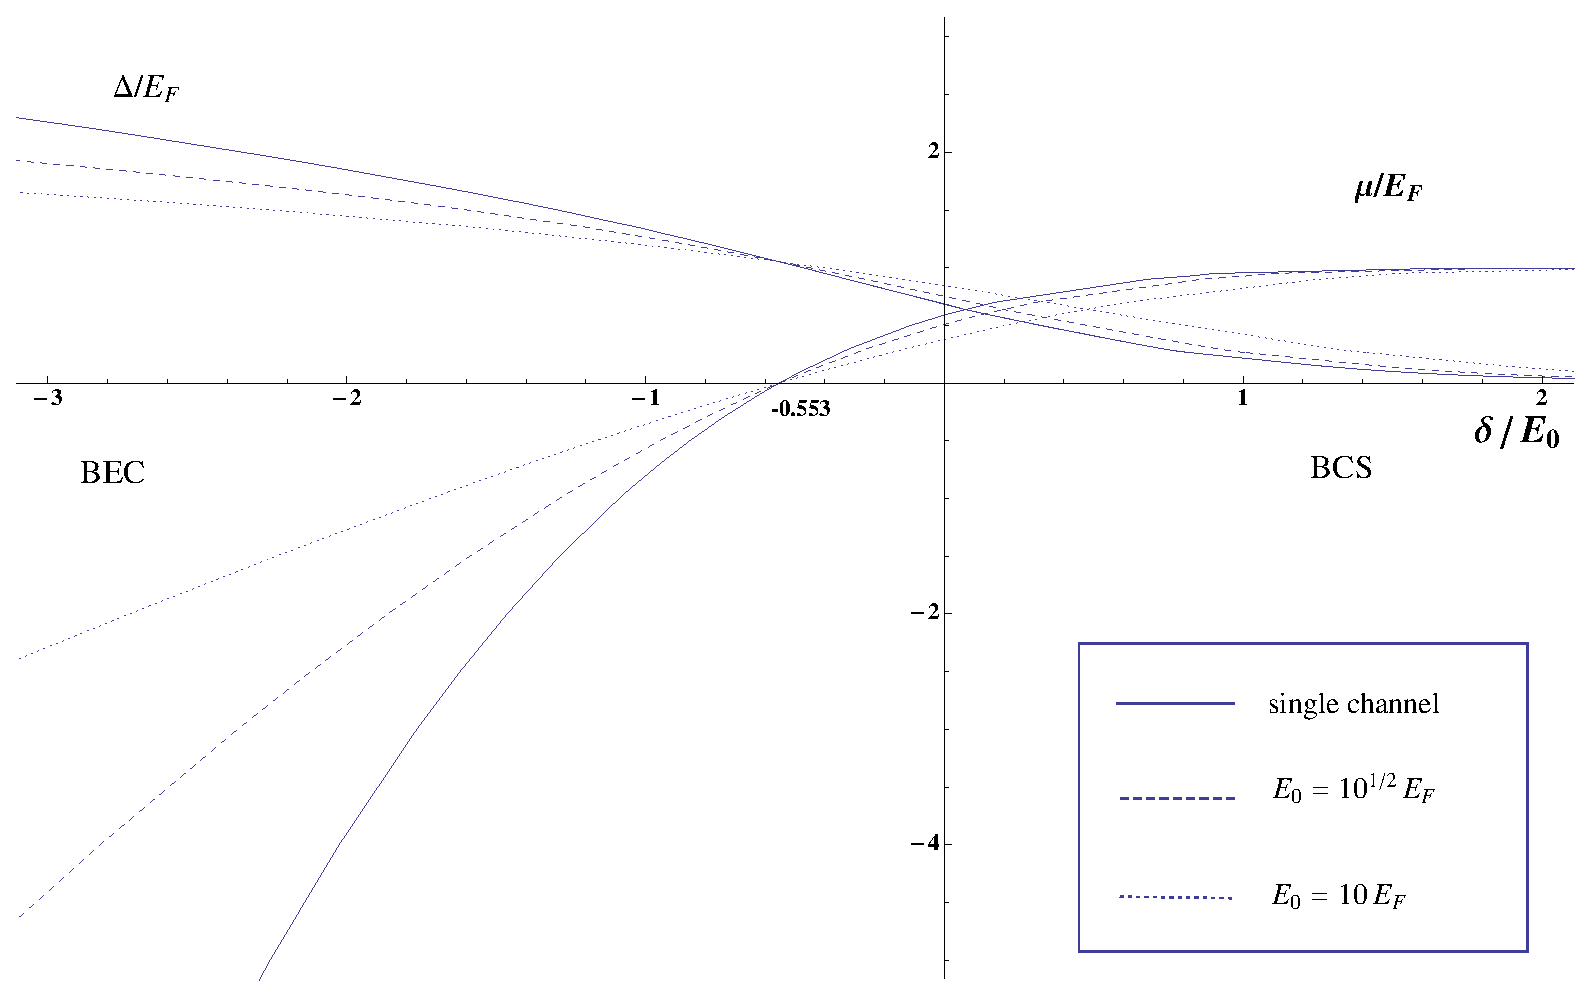
\includegraphics[width=0.8\textwidth]{simpleNarrowMuDt}
\caption{The chemical potential $\mu$ and gap $\Delta$  over crossover with the Feshbach resonance of different $\delta_{c}$} 
\label{fig:pathInt2:simpleNarrowMuDt}
\parbox{0.8\textwidth}{\small  Here $E_{0}=a_{\text{bg}}\mathcal{K}k_{F}$.  $\delta_{c}={E_{0}^{2}}/{E_{F}}$. So the two dashed lines correspond to $\delta_{c}=10E_{F}$ and $100E_{F}$. Notice that $E_{F}$ and $k_{F}$ here are referred to the open-channel quantities. }
\end{center}
\end{figure}
In Fig. \ref{fig:pathInt2:simpleNarrowMuDt}, $\delta_{c}={E_{0}^{2}}/{E_{F}}$, we see the two lines correspond to $\delta_{c}=10E_{F}$ and $100E_{F}$.  Notice that all scales in Fig. \ref{fig:pathInt2:simpleNarrowMuDt} is related the Fermi energy and the Fermi momentum of atoms only in the open-channel.  It is important to find the relation between the open-channel density and the closed-channel density.   Let us look at the open-channel gap equation Eq. \ref{eq:pathInt2:mfopen} 
\begin{equation}
\Delta_{1\vp}=\sum_{\vk}{}U_{\vp\vk}h_{1\vk}+\sum_{\vk}{}Y_{\vp\vk}h_{2\vk}\tag{\ref{eq:pathInt2:mfopen}}
\end{equation}
Not far away from the resonance, the second term dominates the first term.  And considering Eq. \ref{eq:pathInt2:hphi}, $h_{2\vk}=\alpha\phi^{}_{0\vk}u_{\vk}^{2}$, it is not hard to see that the closed-channel normalization factor $\alpha$ is proportional to $\Delta_1$.   At the BEC end, i.e. negative detuning, the closed-channel density increases as $\Delta_1$ increases and eventually dominates the open-channel density.  In fact, for total density $n$, when the closed-channel dominates, $\alpha\approx\sqrt{N}$ and $\Delta_1$ saturates and is directly proportional to the square root of the total density.  
\begin{equation}
\Delta_1\approx\sqrt{N}\sum_{\vk}{}Y_{\vp=0,\,\vk}\phi^{}_{0\vk}u_{\vk}^{2}\approx{\sqrt{n_{\text{total}}}\Delta_{1,\text{sat}}^{(0)}}
\end{equation}
Here the coefficient $\Delta_{1,\text{sat}}^{(0)}$ is common for one specific Feshbach resonance.   
 At such region, the open-channel density is very small.  Fig. \ref{fig:pathInt2:simpleNarrowMuDt} shows $\Delta_1/E_{F,\text{open}}$ increases toward BEC end.  Given the total density,  this increase is   not because $\Delta_{1}$ increases, but because the open-channel density decreases quickly.  Nevertheless, for the large negative detuning, where this formula applies, the chemical potential is most likely negative and the fermionic excitation modes are $\sqrt{\mu^{2}+\Delta_{1}^{2}}$ instead of simple $\Delta_{1}$.  Furthermore, the more important low-energy excitation modes in such systems are most likely to be the bosonic ones.    
 
Corrections to the equations in the second step are all in the order of $\zeta=\Delta_2^2/\eta\Delta_1$.  Given the non-singular nature of the crossover problem, we expect the correction to various quantities are in the same order of $\zeta$. 



There are three distinct length scales in the problem.  The range of the potential, $r_c$, is the smallest.  The intra-channel and inter-channel potentials are  essentially zero outside this range. Potentials energy dominate the kinetic energy in this range and the correlation (wave function) is totally governed by the potential and might have large oscillation.   The two-body correlation follows the two-body wave function in this range.  The second range is the size of the closed-channel bound-state, $a_c$.  The closed-channel bound state only has negligible weight outside this range.  In this range, the many-body correlation still follow the two-body wave function in the closed-channel.  We assume that the closed-channel is high excitation state and therefore has most weight in this region.  The inter-channel Pauli exclusion are mostly accounted in this  region.  Not surprisingly, this region contributes most in the integral of $\lambda_{1}$ and $\lambda_{2}$. When much larger than $a_c$, many-body effect is important. However, the closed-channel has only negligible weight in it and therefore only the open-channel needs to be considered.  



%\section{Mean field result}
 Use the same techniques as Eq. (\ref{eq:pathInt:diffTr}), we have two equations for $D_{1}$ and $D_{2}$,
 \begin{align}
\frac{\delta}{\delta{}D_{1}}:&\qquad&
(\tilde{U}^{-1})_{11}\bar{D}_{1}+(\tilde{U}^{-1})_{21}\bar{D}_{2}-\tr\mbr{{G_{0}}\cdot\cmtrx{0&1&0\\0&0&0\\0&0&0}}=0\\
\frac{\delta}{\delta{}D_{2}}:&\qquad&
(\tilde{U}^{-1})_{12}\bar{D}_{1}+(\tilde{U}^{-1})_{22}\bar{D}_{2}-\tr\mbr{{G_{0}}\cdot\cmtrx{0&0&1\\0&0&0\\0&0&0}}=0
 \end{align}


 If we take $D$ as real constant\footnote{Actually $D_{2}{_{\vk}}$ cannot be constant at high momentum.  However, for the momentum we are interested, i.e. the momentum lower or in the order of Fermi momentum, it slowly varies.  Therefore  it is reasonable to take it as constant.},     we can find the mean field result.  Usting Eq. (\ref{eq:pathInt2:Gexpand}),
 
 \begin{equation}\label{eq:pathInt2:G0}
 \begin{split}
 G_{0}=&
 \begin{pmatrix}
 {g_{1\,\vk}}&
-u_{k}v_{k}{g_{2\,\vk}}&0\\
-u_{k}v_{k}{g_{2\,\vk}}& {g_{3\,\vk}}&0\\
  0&0&\nth{i\omega_{n}-\xi_{3}{}_{\vk}}
 \end{pmatrix}\\
&+\frac{D_{2}}{\eta}
\begin{pmatrix}
\frac{D_{1}^{2}D_{2}}{4E_{\vk}^{3}}g_{2\,\vk}&\frac{D_{1}D_{2}\xi_{\vk}}{4E_{\vk}^{3}}g_{2\,\vk}&-g_{1\,\vk}+\nth{i\omega_{n}-\xi_{3}{}_{\vk}}\\
\frac{D_{1}D_{2}\xi_{\vk}}{4E_{\vk}^{3}}g_{2\,\vk}&-\frac{D_{1}^{2}D_{2}}{4E_{\vk}^{3}}g_{2\,\vk}&u_{k}v_{k}{g_{2\,\vk}}\\
-g_{1\,\vk}+\nth{i\omega_{n}-\xi_{3}{}_{\vk}}&u_{k}v_{k}{g_{2\,\vk}}&0
\end{pmatrix}
\end{split}
 \end{equation}
\begin{gather}
g_{1}{}_{\vk}=\frac{u_{\vk}^{2}}{i\omega_{n}-\xi_{1}{}_{\vk}}+\frac{v_{\vk}^{2}}{i\omega_{n}-\xi_{2}{}_{\vk}}\\
g_{2}{}_{\vk}=\nth{i\omega_{n}-\xi_{1}{}_{\vk}}-\nth{i\omega_{n}-\xi_{2}{}_{\vk}}\\
g_{3}{}_{\vk}=\frac{v_{\vk}^{2}}{i\omega_{n}-\xi_{1}{}_{\vk}}+\frac{u_{\vk}^{2}}{i\omega_{n}-\xi_{2}{}_{\vk}}
\end{gather}

 \begin{align}
\tr\mbr{G_{0}\cdot\cmtrx{0&1&0\\0&0&0\\0&0&0}}&=
\sum_{\vk}\sum_{\omega_{n}}
	\mbr{(\nth{i\omega_{n}-\xi_{1}{}_{\vk}}-\nth{i\omega_{n}-\xi_{2}{_{\vk}}})
	(-\frac{D_{1}}{2E_{\vk}}+\frac{D_{1}D_{2}^{2}\xi_\vk}{4E_{\vk}^{3}\eta})}\\
	&=\sum_{\vk}(\frac{D_{1}}{2E_{\vk}}-\frac{D_{1}D_{2}^{2}\xi_\vk}{4E_{\vk}^{3}\eta})\\
\tr\mbr{G_{0}\cdot\cmtrx{0&0&1\\0&0&0\\0&0&0}}&=
\sum_{\vk}\sum_{\omega_{n}}
\mbr{\nth{i\omega_{n}-\xi_{3}{}_{\vk}}-
\frac{u_{\vk}^{2}}{i\omega_{n}-\xi_{1}{}_{\vk}}-\frac{v_{\vk}^{2}}{i\omega_{n}-\xi_{2}{}_{\vk}}}\frac{D_{2}}{\eta}\label{eq:pathInt2:F20}\\
&=\sum_{\vk}\frac{D_{2}}{\eta}u_{\vk}^2
  \end{align}
Here we take the interest only in $T=0$, so we only need to consider the negative frequencies ($\xi_{2\,\vk}$, $\xi_{3\,\vk}$) for summation of Matsubara frequency. Note that the second summation diverges badly in high-momentum. %this is because we take $D_2$ as constant.  It decreases at high-energy in the scale of $\eta$ and needs to be regularize carefully.  
We notice that this term is controlled by parameter $D_{2}/\eta$, this actually goes back to the fact that we only keep the first order in $L$ expansion (Eq. \eqref{eq:pathInt2:L1}), which is only valid for energy smaller or in order of Fermi energy.  In a more careful study, this term should be like $D_{2}/(\epsilon_{k}+\eta)$, is approximately $D_{2}/\eta$ when the interesting region  is lower or at the Fermi energy.   We can reestablish the $F_{k}\propto1/\epsilon_{k}$ if we retain all terms in the expansion of $L$, i.e. inverting Green's function $G$ exactly.       Indeed it should be just proportional to simple bounded two-body solution of isolated close-channel, $\phi_{0\,\vk}$ at high-momentum, which is not of interest for the many-body problem. 
 Another interesting thing about this term is the $u_\vk$ factor, which is small below chemical potential $\mu$ in BCS side.  This shows the fact that the low momentum is filled mostly by open-channel and close-channel is crowded out.  However, this does not affect close-channel too much as it is much more extended in momentum space and its occupation over each level is low due to the smaller size of close-channel bound state.  With above result, we can rewrite gap equations as 
\begin{equation*}
\tilde{U}^{-1}D-\mtrx{\sum_{\vk}(\frac{D_{1}}{2E_{\vk}}-\frac{D_{1}D_{2}^{2}\xi_\vk}{4E_{\vk}^{3}\eta})\\\sum_{\vk}\frac{D_{2}}{\eta}u_{\vk}^2}=0
\end{equation*}
 We can multiply it with $\tilde{U}$ and we have 
\begin{equation}\label{eq:pathInt2:meanfield}
\mtrx{D_1\\D_2}=\mtrx{U&Y\\Y^{*}&V}\sum_{\vk}\mtrx{\frac{D_{1}}{2E_{\vk}}-\frac{D_{1}D_{2}^{2}\xi_\vk}{4E_{\vk}^{3}\eta}\\
\frac{D_{2}}{\eta}u_{\vk}^2}
\end{equation}
 This equation can be renormalized in a very similar fashion as variation method. Notice that the second term in the first component describes the Pauli exclusion between two channels.  

\subsection{Renormalizing mean-field equation\label{sec:pathIntRenorm}}
We define two quantities for the summand in the mean-field equation Eq. \ref{eq:pathInt2:meanfield}.
\begin{gather}
F_{1\,\vk}=\frac{D_{1}}{2E_{\vk}}-\frac{D_{1}D_{2}^{2}\xi_\vk}{4E_{\vk}^{3}\eta}\\
F_{2\,\vk}=\frac{D_{2}}{\eta}u_{\vk}^2\label{eq:pathInt2:F2k}
\end{gather}
Considering the argument from last section, we modify equation of $F_2$ to the following,
\begin{equation}
\tilde{F}_{2\,\vk}=\frac{D_{2}}{\eta+2\epsilon_{\vk}}u_{\vk}^2\label{eq:pathInt2:F2kMod}
\end{equation}
And now $F_2$ has the same behavior at high momentum as $F_1$, actually this is the behavior we expected for $\epsilon_k<\eta$, it falls off even faster beyond energy scale of $\eta$, which is determined by the specific shape of close-channel potential.

We can rewrite the mean-field equation as
\begin{gather}
D_{1}=\sum_{\vk}(U F_{1\,\vk}+Y \tilde{F}_{2\,\vk})\label{eq:pathInt2:D2}\\
D_{2}=\sum_{\vk}(Y^{*} F_{1\,\vk}+V \tilde{F}_{2\,\vk})\label{eq:pathInt2:D2}
\end{gather}
Here we see the $F_{1\,\vk}$ and $\tilde{F}_{2}$  both go as $1/\epsilon_{\vk}$  at high-momentum.  %To resolve divergence in the summation of $F_{2\,\vk}$ we restore the momentum dependence on $D_{2\,\vk}$ and therefore $F_{2\,\vk}$.  
  And we can see $\frac{D_{2}}{\eta}$ is actually a good approximation at low-momentum, where kinetic energy is much smaller than $\eta$.  We can rewrite $\tilde{F}_{2}=\alpha\phi_{0\,\vk}u_{\vk}^{2}$. Eq. (\ref{eq:pathInt2:D2}) can be rewritten as
\begin{equation*}
\eta{}F_{2\,\vp}=\sum_{\vk}(Y^{*} F_{1\,\vk}+V F_{2\,\vk})\label{eq:pathInt2:D2}
\end{equation*}
comparing this to a two-body \sch equation
\begin{equation}
-E_{0}\phi_{0\,\vp}=\epsilon_{\vp}\phi_{0\,\vp}-\sum_{\vk}V \phi_{0\,\vk}
\end{equation}
where $E_{0}$ is the binding energy of two-body bound state of isolated close-channel.   




\chapter{Excitation modes\label{ch:excitation}}
In the single channel crossover, fermionic modes are related to the two-body correlation of the original fermions; while the bosonic modes are related to the two-body correlation of the auxiliary new bosonic fields (order parameters $(\Delta_{1}, \Delta_{2})$).  Similarly to the single-channel case, most modes are gapped with minimum at  $\Delta_{1}$ and only one  Goldstone mode for the (in-phase) phase fluctuation of order parameters (bosonic fields) is gapless with linear dispersion at low energy. 
\section{Fermionic excitation modes and Bogoliubov transformation\label{sec:pathInt2:bog}}
If we limit ourselves in the mean field level, we can interpret the transformation $T_\vk{}L_\vk$ in Eq. \eqref{eq:pathInt2:B} as the Bogoliubov canonical transformation, while  the $3\times3$ fermionic correlation matrix $B$ in Eq. (\ref{eq:pathInt2:Bapprox}-\ref{eq:pathInt2:xiExpand3}) gives us the spectrum of the  fermionic quasi-particle excitation. From Eq. \eqref{eq:pathInt2:actionMix} and Eq. \eqref{eq:pathInt2:B}, the action is diagonal for new fermions (quasi-particles) field 
\begin{equation*}
\Phi_\vk\equiv\mtrx{\phi_{\text{\Rmnum{1}},+\vk}\\\bar\phi_{\text{\Rmnum{2}},-\vk}\\\bar\phi_{\text{\Rmnum{3}},-\vk}}
=L^{\dg}_{\vk}T^{\dg}_{\vk}\mtrx{\psi_{a\,\vk}\\\bar\psi_{b\,-\vk}\\\bar\psi_{c\,-\vk}}
\end{equation*}
Putting the above transformation into the operator language and using $\mathcal{X}_{\text{I}}$, $\mathcal{X}_{\text{II}}$, and $\mathcal{X}_{\text{III}}$ to denote the new quasi-particles,  we have the relation 
\begin{equation}
\mtrx{\mathcal{X}^{}_{\text{\Rmnum{1}},+\vk}\\\mathcal{X}_{\text{II},-\vk}^{\dg}\\\mathcal{X}_{\text{III},-\vk}^{\dg}}
=L^{\dg}_{\vk}T^{\dg}_{\vk}  \mtrx{a_{\vk}\\b_{-\vk}^{\dg}\\c_{-\vk}^{\dg}}
\end{equation}   

\begin{equation}\tag{\ref{eq:pathInt2:T}}
T_k=\mtrx{u_k&v_k&0\\-v_k&u_k&0\\0&0&1}
\end{equation}
\begin{equation}\tag{\ref{eq:pathInt2:L1}}
L_{\vk}\approx{}I+
\mtrx{0&-\frac{\Delta_{1}{}\Delta_{2}{}}{4E^{2}_{\vk}}&u_{\vk}\\
\frac{\Delta_{1}{}\Delta_{2}{}}{4E^{2}_{\vk}}&0&v_{\vk}\\
-u_{\vk}&-v_{\vk}&0
}\frac{\Delta_{2}{}}{\eta}
\equiv{}I+\delta_{k}\qquad
L^{\dg}_{\vk}=I-\delta_{\vk}
\end{equation}
First of all, mixture of $a_{\vk}$ and $b^{\dg}_{-\vk}$ ($c^{\dg}_{-\vk}$) indicates the pairing of atoms of the opposite momentum. Furthermore,   mixture of creators and annihilators dictates the approach of the grand-canonical ensemble, i.e., the ground state is a number non-conserved state.   Secondly, $L$ matrix cannot be separated into two channels, which indicate the mixture of two channels.   At the mean field level, both $\Delta_{1}$ and $\Delta_{2}$ are taken as real constants.  The new Hamiltonian at this level is 
\begin{equation}
\hat{H}=f(\Delta_{1},\Delta_{2})+E_{1\,\vk}\mathcal{X}^{\dg}_{\text{I},+\vk}\mathcal{X}^{}_{\text{I},+\vk}
+E_{2\,\vk}\mathcal{X}^{\dg}_{\text{II},-\vk}\mathcal{X}^{}_{\text{II},-\vk}
+E_{3\,\vk}\mathcal{X}^{\dg}_{\text{III},-\vk}\mathcal{X}^{}_{\text{III},-\vk}
\end{equation}
And the spectrum is just like we calculated in Sec. \ref{sec:diagonalGreen}, Eqs. \ref{eq:pathInt2:xiExpand}-\ref{eq:pathInt2:xiExpand3}.  We quote here again
\begin{align}
E_{1\vk}&\equiv{}E_{\vk}+\gamma_{1\vk}\approx{}E_{\vk}+u_{\vk}^{2}\zeta\tag{\ref{eq:pathInt2:xiExpand}}\\
E_{2\vk}&\equiv{}E_{\vk}+\gamma_{2\vk}
\approx{}E_{\vk}-v_{\vk}^{2}\zeta\tag{\ref{eq:pathInt2:xiExpand2}}\\
E_{3\vk}&\equiv{}\xi_{\vk}+\eta+\gamma_{3\vk}\approx{}\epsilon_{\vk}+\eta+\frac{\zeta}{2}
\tag{\ref{eq:pathInt2:xiExpand3}}
\end{align}
Here $\gamma_{1}$, $\gamma_{2}$ and $\gamma_{3}$ are correction due to the inter-channel Pauli exclusion. 

This clearly shows that $\mathcal{X}^{\dg}_{\text{I},\vk}$, $\mathcal{X}^{\dg}_{\text{II},\vk}$, and $\mathcal{X}^{\dg}_{\text{III},\vk}$ are fermionic quasi-particle excitation modes with spectrum $E_{i\,\vk}$ and   $L^{\dg}_{\vk}T^{\dg}_{\vk}$ is  the Bogoliubov canonical transformation to transfer the normal fermionic modes into these elementary quasi-particle modes .  Here we see in the excitation, different species of opposite momentum, $(a,b)$ and $(a,c)$, mixed together to form the elementary excitation due to the paring in the ground state.  
  From Eqs. (\ref{eq:pathInt2:xiExpand}-\ref{eq:pathInt2:xiExpand3}), we see that the fermionic excitation modes basically follow the pattern in the broad resonance.  In the broad resonance where the closed-channel only modifies the interaction in the open-channel,  there are basically three fermionic quasi-particle modes: two (degenerate) Bogoliubov quasi-particle modes  in the open-channel, $E_{\vk}=\sqrt{\xi^{2}_{\vk}+\Delta_{1}^{2}}$ as in BCS theory (gapped at $\Delta_{1}$ in the BCS-like states, $\mu>0$ and ${\sqrt{\mu^{2}+\Delta_{1}^{2}}}$ in the BEC-like states, $\mu<0$)  
; and one high fermionic excitation mode in the closed-channel, $\xi_{\vk}+\eta$, as in normal gas.  In the narrow resonance, first of all, the gap $\Delta_{1}$ (or $\sqrt{\mu^{2}+\Delta_{1}^{2}}$) itself is modified  by consideration of the extra Pauli exclusion with the correction in the  order of $\zeta$.  Once that is taken into account, the above conclusion is approximately correct except high-order corrections in $\zeta$.   The originally double degenerate excitation modes, $E_{\vk}=\sqrt{\xi^{2}_{\vk}+\Delta_{1}^{2}}$ , now split by $\zeta\Delta_{1}$; while the third high excitation corresponding the normal fermionic excitation in the closed-channel has a small correction in the same order.   On the other respect, as discussed earlier in Sec. \ref{sec:diagonalGreen}, these corrections are due to the inter-channel Pauli exclusion and do not vanish when the inter-channel coupling, $Y$, approaches zero.  

\section{Collective excitation modes}
Fermionic modes are derived from the correlation function $\nG$ of the fermion fields $\Psi$, and therefore are mostly single (quasi)particle like.  On the other hand, order parameters ($\Delta_{1}$, $\Delta_{2}$) are defined in terms of collective behavior of many fermion atoms.  Fluctuations of order parameters thus marked the collective excitation modes of the system. Here with a two-component order parameter, four independent modes exist:   two for magnitude variation of each $\Delta_i$,  internal phase between two $\Delta_i$, and the overall local phase $\theta(x)$ of $\Delta_1$ and $\Delta_2$.  The first three change the magnitude of action and therefore massive; while the last one leaves the action invariant and thus massless.  
  For the single-channel crossover, Sec. \ref{sec:collective1} considers all (magnitude and phase) modes of the order parameter fluctuation at the same time, and only calculates  the low sound-like part of the spectrum. In the two-channel case, a general analysis with all modes in becomes unwieldy.  
We instead focus on one mode a time. We isolate the change in one mode and leave others at their mean-field values.  

Phase fluctuations are usually more interesting, the in-phase mode is the counterpart of the Anderson-Bogoliubov modes in the single channel problem, while the two channels introduce a new out-of-phase mode. We study two phase fluctuation modes in the next two sections. 
\subsection{The in-phase phase fluctuation }
The action of $\Delta$, $S(\bar{\Delta}_i,\Delta_i)$ (Eqs. \ref{eq:pathInt2:nG}, \ref{eq:pathInt2:actionD}), is invariant if the phases of $\Delta_{1\,\vk}$ and $\Delta_{2\,\vk}$ rotate simultaneously. We therefore conclude that there exists a massless (Goldstone) mode corresponding to the local phase invariance.We first study the massless two-channel in-phase phase fluctuation.   Introduce the phase fluctuation $\theta$, 
\begin{equation*}
\Delta_{i}(x)\rightarrow{}\Delta_{i}e^{i2\theta(x)}\qquad{}
\bar{\Delta}_{i}(x)\rightarrow{}\bar{\Delta}_{i}e^{-i2\theta(x)}
\end{equation*}
This is equivalent to  phase  rotation of fermionic variable $\psi$
\begin{equation*}
\psi_{i}(x)\rightarrow{}\psi_{i}(x)e^{i\theta(x)}\qquad{}
\bar{\psi}_{i}(x)\rightarrow{}\bar{\psi}_{i}(x)e^{-i\theta(x)}
\end{equation*}
Again, the phase $\theta(x)$ is common for the both components.   With a phase shift, we can rewrite the action (taken mean-field value $\Delta^{(0)}=(\Delta_1,\Delta_2)^\dg$) (here we  follow treatment of Nagaosa\cite{Nagaosa})
\begin{subequations}\label{eq:pathInt2:actionPhase}
\begin{align}
S[\theta,\bar\psi_{i},\psi_{i}]=&S_0[\bar\psi_{i},\psi_{i}]+S_1[\theta,\bar\psi_{i},\psi_{i}]+S_2[\theta,\bar\psi_{i},\psi_{i}]\\
S_0[\bar\psi_{i},\psi_{i}]=&\int{dx}
\Big\{\sum_{j}\bar\psi_{j}(\partial_\tau-\nth{2m}\nabla^{2}-\mu+\eta_{j})\psi_{j}\nonumber\\
&\quad+\Delta^{(0)}{}^{\dg}\tilde{U}^{-1}\Delta^{(0)}-(\bar\psi\bar\psi)\Delta^{(0)}-{\Delta^{(0)}}{}^{\dg}(\psi\psi)\Big\}\\
S_1[\theta,\bar\psi_{i},\psi_{i}]=&\int{dx}\sum_{j}\Big\{
   i\,\bar\psi_{j}(\partial_{\tau}\theta)\psi_{j}+\nabla\theta\cdot\nth{2mi}[\bar\psi_{j}\nabla\psi_{j}-(\nabla\bar{\psi}_{j})\psi_{j}]\Big\}\\
S_2[\theta,\bar\psi_{i},\psi_{i}]=&\int{dx}\sum_{j}\nth{2m}(\nabla\theta)^{2}\bar\psi_{j}\psi_{j}
\end{align}
\end{subequations}
Note that here $\Delta^{(0)}$ is a constant 2-component vector, no longer a functional variable.  Here we see that $S_{0}$ has the same form as before except it only takes the mean field value of $\Delta$ and it is described by the same correlation $G_{0}$ (Eq. \ref{eq:pathInt2:nG}).  We can regard $S_{1}$ and $S_{2}$ as perturbation for the so-called gradient expansion on $\nabla\theta$.  It is then obvious that $S_{1}$ is in the first order while $S_{2}$ is in the second order regarding with the (time or space) derivative of $\theta$.  Use the same spinor representation as before, $S$ is bilinear of $\psi$ and therefore we can formally integrate out $\psi$. 
\begin{equation}
S[\theta]=const.+\ln\det\nG(\theta)
\end{equation}
 We write out the formal Green function according to the above action (with respect to the Nambu-like spinor)
\begin{subequations}
\begin{align}
\nG=&G_{0}^{-1}+K_{1}+K_{2},\\
K_{1\, k,k'}=
	&\nth{({\beta{}V)}^{1/2}}(\omega_n-\omega_{n'})\theta(k-k')\sigma_3+
		\nth{{(\beta{}V)}^{1/2}}i\frac{(\vk-\vk')\cdot(\vk+\vk')}{2m}\theta(k-k')\hat{1}\\
K_{2\, k,k'}=
	&\nth{2m}\sum_{q,q'}\nth{{\beta{}V}}(\vq\cdot\vq')\theta(q)\theta(q')\delta(q+q'+k-k')\sigma_3
\end{align}
\end{subequations}
where $G_{0}$ is the same as (Eqs. \ref{eq:pathInt2:nGDelta}, \ref{eq:pathInt2:nG}).  Here $k=(\omega_n,\vk)$ and $k'=(\omega_{n'},\vk')$.  And like in the single channel, 
\begin{equation}
\sigma_3=\mtrx{1&0&0\\0&-1&0\\0&0&-1}
\end{equation}
and $\hat{1}$ is $3\times3$ identity matrix.  As the expansion in Eq. \ref{eq:pathInt:expand}, we can look for the expansion of $\nG$ over $K_{1,2}$.  
\begin{equation}\tag{\ref{eq:pathInt:expand}}
\tr\ln \nG=\tr\ln\hat{G_{0}}^{-1}+\tr(\hat{G_{0}}\hat{K})-\nth{2}\tr(\hat{G_{0}}\hat{K}\hat{G_{0}}\hat{K})+\cdots
\end{equation}
For the first order, $\tr(\hat{G_{0}}\hat{K})$, 
\begin{align}
\tr(\hat{G_{0}}\hat{K_1})=&\sum_{k}{G_{0\,k}K_{1\,k,k}}=0\\
\tr(\hat{G_{0}}\hat{K_2})=&\sum_{k}{G_{0\,k}K_{2\,k,k}}\nonumber\\
	=&-\nth{2m}\nth{{\beta{}V}}\sum_{k}\tr(\hat{G}_{0\,k}\sigma_3)\sum_{q}q^2\theta{q}\theta{-q}\nonumber\\
	=&-\frac{n}{2m}\sum_{q}q^2\theta{(q)}\;\theta{(-q)}
\end{align}
Here we use the fact $\nth{{\beta{}V}}\sum_{k}\tr(\hat{G}_{0\,k}\sigma_3)=n$. $\tr(\hat{G_{0}}\hat{K_2})$ is already in the second order of $\theta$, and we only need to keep the expansion of $K_2$ to this order. On the other hand, we have to go to the second order of $K_1$ for the second order of $\theta$. 
\begin{align}		
\tr(\hat{G_{0}}{K_1}\hat{G_{0}}{K_1})=&\sum_{k,q}\tr(\hat{G}_{0,k+q}K_{1\,k+q,k}\hat{G}_{0\,k}K_{1\,k,k+q})\label{eq:pathInt2:GKGK}\\
=&\nth{{\beta{}V}}\sum_{k,q=(\omega_m,\vq)}\theta(q)\theta(-q)\Big[(-\omega_m^2)\tr(\hat{G}_{0,k+q}\sigma_3\hat{G}_{0\,k}\sigma_3)\nonumber\\
&\quad+\nth{m^2}\sum_{i,j=(x,y,z)}q_iq_j(k_i+\frac{q_i}{2})(k_j+\frac{q_j}{2})\tr(\hat{G}_{0,k+q}\hat{G}_{0\,k})\Big]\label{eq:pathInt2:GKGK2}\\
\equiv&\sum_{q}\theta(q)\theta(-q)\big[-\pi^{(0)}(q)\omega_m^2+\sum_{i,j=(x,y,z)}\pi^{(\perp)}_{ij}(q)q_iq_j\big]\label{eq:pathInt2:pi}
\end{align}
Here we introduce $q=(\omega_m,\vq)=k-k'$.  \emph{We can take $q=0$ in $\pi^(0)(q)$ and $\pi^{(\perp)}(q)$ for low frequency and momentum ($\omega_m,\nth{2m} |\vq|^2\ll\Delta_{1,2}$).  } Use the previous result of Sec. \ref{sec:diagonalGreen}, we can calculate the Green's function in the lowest and first order of $\zeta$ in $\pi$'s.  After some long but straightforward algebra (see Appendix. \ref{sec:calculatePi}), we find
\begin{gather}
\pi^{(0)}(0)\approx\sum_{\vk}\frac{\Delta_{1}^{2}}{E_{\vk}^{3}}
	-\sum_{\vk}\frac{\Delta_{1}^{2}\Delta_{2}^{2}\xi_{\vk}}{2E_{\vk}^{5}(\xi_{\vk}+\eta)}
\label{eq:pathInt2:pi0}\\
\pi^{(\perp)}(0)=0
\end{gather}
Combining all these together, we have a new action for the phase fluctuation $\theta$
\begin{equation}
S[\theta]=\int{dx}\sum_{q}\theta(q)\theta(-q)\big[\nth{2}\pi^{(0)}(0)\omega_m^2-\frac{n}{2m}q^2\big]
\end{equation}
The correlation determines the velocity of the Anderson-Bogoliubov collective mode.  The second term in Eq. \eqref{eq:pathInt2:pi0}, $-\sum_{\vk}\frac{\Delta_{1}^{2}\Delta_{2}^{2}\xi_{\vk}}{2E_{\vk}^{5}(\xi_{\vk}+\eta)}\approx-\sum_{\vk}\frac{\Delta_{1}^{3}}{2E_{\vk}^{3}}\frac{\xi_{\vk}}{E_{\vk}}\nth{E_{\vk}}\zeta$, is the only correction in the next order.  Thus its behavior is qualitatively same as  single-channel with some correction in the order of $\zeta\ll1$ (see Appendix \ref{sec:pathApp:consistency}).


\subsection{The out-of-phase phase fluctuation}
Another interesting phase fluctuation of order parameters is the  phase fluctuation in two channels out of phase.  This mode is unique for a two-channel system without any counterpart in the single-channel modal.  When  the phase fluctuation of two channels are out of  sync,  the inter-channel coupling changes.  Thus, it is  expected to be  a gapped (massive) mode.  Similar as the in-phase mode,  we narrow down to the mode that the phases of two atoms  ($\psi_{b}$ and $\psi_{c}$) are opposite and leave all other modes constant.  
\begin{equation*}
\mtrx{\psi_{a}(x)\\\psi_{b}(x)\\\psi_{c}(x)}\rightarrow{}
	\mtrx{\psi_{a}(x)\\\psi_{b}(x)e^{+i\theta(x)}\\\psi_{c}(x)e^{-i\theta(x)}}
\qquad{}
\mtrx{\bar\psi_{a}(x)\\\bar\psi_{b}(x)\\\bar\psi_{c}(x)}\rightarrow{}
	\mtrx{\bar\psi_{a}(x)\\\bar\psi_{b}(x)e^{-i\theta(x)}\\\bar\psi_{c}(x)e^{+i\theta(x)}}
\end{equation*}
The order parameters do not have a simple transformation because they are connected to two channels via $2\times2$ interaction matrix $\tilde{U}$, which mix two channels (Eq. \ref{eq:pathInt2:DeltaPhi}).  
\begin{equation*}
\begin{pmatrix}\Delta_{1}(x)\\\Delta_{2}(x)\end{pmatrix}\rightarrow{}
	\mtrx{U&Y\\Y^{*}&V}\begin{pmatrix}\psi_{b}\psi_{a}(x)e^{+i\theta(x)}\\\psi_{c}\psi_{a}(x)e^{-i\theta(x)}\end{pmatrix}
%	=\begin{pmatrix}\Delta_{1}^{(0)}(x)\\\Delta_{2}^{(0)}(x)\end{pmatrix}+
%	\mtrx{U&Y\\Y^{*}&V}\begin{pmatrix}\av{\psi_{b}\psi_{a}}(x)(e^{+i\theta(x)}-1)\\\av{\psi_{c}\psi_{a}}(x)(e^{-i\theta(x)}-1)\end{pmatrix}
	%\approx\mtrx{U&Y\\Y^{*}&V}\mtrx{\psi_{b}\psi_{a}(x)(1+i\theta)\\\psi_{b}\psi_{a}(x)(1-i\theta)}
\end{equation*}
This term cannot be easily written in terms of mean-field value $\Delta_i$.   On the other hand, as mentioned before, we freeze all  other modes to their mean-field value except $\theta$.  We therefore adopt another pair $({\psi_{b}\psi_{a}},{\psi_{c}\psi_{a}})$, which is the linear recombination of $(\Delta_{1},\Delta_{2})$.  
%On the other hand, we do not have a full two-dimensional functional variables $\Delta_i$. 
%\begin{equation*}
%\begin{pmatrix}\bar\Delta_{1}(x)&\bar\Delta_{2}(x)\end{pmatrix}\rightarrow{}
%	\begin{pmatrix}\bar\Delta_{1}(x)e^{-i\theta(x)}&\bar\Delta_{2}(x)e^{+i\theta(x)}\end{pmatrix}
%\end{equation*}

%The original action can be expended in the similar fashion as Eq. \ref{eq:pathInt2:actionPhase}. Indeed it is almost the same except there is one more terms due to inter-channel coupling term.  
%\begin{align*}
%&\Delta^{(0)}{}^{\dg}\tilde{U}^{-1}\Delta^{(0)}-(\bar\psi\bar\psi)\Delta^{(0)}-{\Delta^{(0)}}{}^{\dg}(\psi\psi)\\
%=&\bar\Delta^{(0)}_{1}{}^{\dg}\tilde{U}^{-1}_{11}\Delta^{(0)}_{1}+\bar\Delta^{(0)}_{2}\tilde{U}^{-1}_{22}\Delta^{(0)}_{2}
%	+\bar\Delta^{(0)}_{1}\tilde{U}^{-1}_{12}\Delta^{(0)}_{2}e^{-i2\theta(x)}
%	+\bar\Delta^{(0)}_{2}\tilde{U}^{-1}_{21}\Delta^{(0)}_{1}e^{+i2\theta(x)}\\
%&-(\bar\psi\bar\psi)\Delta^{(0)}-{\Delta^{(0)}}{}^{\dg}(\psi\psi)\\
%\end{align*}
Comparing to the in-phase phase rotation, the out-of-phase one does modify the action's magnitude. Write the interaction term in the momentum space,
\begin{align*}
&\Delta^{}{}^{\dg}\tilde{U}^{-1}\Delta^{}\\
=&\mtrx{\av{\bar{\psi}_{b}\bar{\psi}_{a}}e^{-i\theta}&\av{\bar{\psi}_{c}\bar{\psi}_{a}}e^{+i\theta}}\tilde{U}^{}\tilde{U}^{-1}\tilde{U}
\mtrx{\av{\psi_{b}\psi_{a}}e^{+i\theta}\\\av{\psi_{c}\psi_{a}}e^{-i\theta}}\\
%=&\mtrx{\av{\psi_{b}\psi_{a}}e^{-i\theta}&\av{\psi_{c}\psi_{a}}e^{+i\theta}}\mtrx{U&Y\\Y^{*}&V}
%\mtrx{\av{\psi_{b}\psi_{a}}e^{+i\theta}\\\av{\psi_{c}\psi_{a}}e^{-i\theta}}
=&\mtrx{\htd_{1}^{*}&\htd_{2}^{*}}\mtrx{U&Ye^{-i2\theta}\\Y^{*}e^{+i2\theta}&V}\mtrx{\htd_{1}\\\htd_{2}}\\
=&\Delta^{(0)}{}^{\dg}\tilde{U}^{-1}\Delta^{(0)}
+\mbr{Y(e^{-i2\theta}-1)\htd_{1}^{*}\htd_{2} +Y^{*}(e^{+i2\theta}-1)\htd_{1}\htd_{2}^{*}}
\end{align*}
Note that here we take the mean-field expectation of pairs of fermions $\tilde{h}_{1}=\av{\psi_{b}\psi_{a}}=\sum_{\vk}h_{1\vk}$, $\tilde{h}_{2}=\av{\psi_{c}\psi_{a}}=\sum_{\vk}h_{2\vk}$, and their complex conjugates\footnote{$\psi\psi$ and $\bar\psi\bar\psi$ are complex conjugate in the mean field.}.  Comparing with the action of the in-phase phase fluctuation (Eq. \ref{eq:pathInt2:actionPhase}), we find one more terms in the new action.  
\begin{subequations}\label{eq:pathInt2:actionPhase2}
\begin{align}
S[\theta,\bar\psi_{i},\psi_{i}]=&S_0[\bar\psi_{i},\psi_{i}]+S_1[\theta,\bar\psi_{i},\psi_{i}]+S_2[\theta,\bar\psi_{i},\psi_{i}]
	+S_3[\theta]\\
S_0[\bar\psi_{i},\psi_{i}]=&\int{dx}
\Big\{\sum_{j=(a,b,c)}\bar\psi_{j}(\partial_\tau-\nth{2m}\nabla^{2}-\mu+\eta_{j})\psi_{j}\nonumber\\
&\quad+\Delta^{(0)}{}^{\dg}\tilde{U}^{-1}\Delta^{(0)}-(\bar\psi\bar\psi)\Delta^{(0)}-{\Delta^{(0)}}{}^{\dg}(\psi\psi)\Big\}\\
S_1[\theta,\bar\psi_{i},\psi_{i}]=&\int{dx}\Big\{
   i\,(\partial_{\tau}\theta)(\bar\psi_{b}\psi_{b}-\bar\psi_{c}\psi_{c})\\
   &\quad+\nabla\theta\cdot\nth{2mi}[\bar\psi_{b}\nabla\psi_{b}-\bar\psi_{c}\nabla\psi_{c}
   -(\nabla\bar{\psi}_{b})\psi_{b}   +(\nabla\bar{\psi}_{c})\psi_{c}]\Big\}\\
S_2[\theta,\bar\psi_{i},\psi_{i}]=&\int{dx}\nth{2m}(\nabla\theta)^{2}(\bar\psi_{b}\psi_{b}+\bar\psi_{c}\psi_{c})\\
S_3[\theta]=&\int{dx}\mbr{Y(e^{-i2\theta}-1)\htd_{1}^{*}\htd_{2} +Y^{*}(e^{+i2\theta}-1)\htd_{1}\htd_{2}^{*}}
\end{align}
\end{subequations}
Let us look at $S_{3}$ first. We can expand it around small $\theta$.  
\begin{align}
S_3[\theta]=&\int{dx}\mbr{Y(e^{-i2\theta}-1)\htd_{1}^{*}\htd_{2} +Y^{*}(e^{+i2\theta}-1)\htd_{1}\htd_{2}^{*}}\\
  =&\int{dx}-i2\mbr{Y\htd_{1}^{*}\htd_{2} -Y^{*}\htd_{1}\htd_{2}^{*}}\theta
  	-2\mbr{Y\htd_{1}^{*}\htd_{2} +Y^{*}\htd_{1}\htd_{2}^{*}}\theta^2
\end{align}



From Eq. \ref{eq:pathInt2:h1}
\begin{equation*}
 h_{1\vk}=\Delta_{1}\frac{E_{1\,\vk}+\xi_{\vk}+\eta}{(E_{1\,\vk}+E_{2\,\vk})(E_{1\,\vk}+E_{3\,\vk})}
\end{equation*}
If $\Delta_{1}=\Delta_{1}e^{i\varphi}$, all $h_{1\vk}$ has argument $\varphi$ (or $\pi+\varphi$). Thus $\htd_{1}$ has argument $\varphi$ (or $\pi+\varphi$) as well.  Also consider the mean-field equation  $\Delta_{1}=U\htd_{1}+Y\htd_{2}$, We can rewrite 
\begin{equation}
Y\htd_{1}^{*}\htd_{2}=\htd_{1}^{*}\Delta_{1}-\htd_{1}^{*}U\htd_{1}
\end{equation}
$U$ is real for a Hermite interaction.  So this quantity is real.  In addition,  $Y^{*}\htd_{1}\htd_{2}^{*}$ is complex conjugate of $Y^{}\htd_{2}\htd_{1}^{*}$. So they are equal because they are both real.  From all these, we conclude that the linear term of $\theta$ vanishes.  This is actually expected for a perturbation around saddle point.  Now we can rewrite this term
\begin{equation}
S_{3}[\theta]=\int{dx}-4Y\htd_{1}^{*}\htd_{2}\theta^{2}=\sum_{q}\theta({q})\theta({-q})(-4Y\htd_{1}^{*}\htd_{2})
\end{equation}
$Y\htd_{1}^{*}\htd_{2}$ is actually the expectation of coupling for the two channel correlation.  It is not hard to see that this value  is negative in the minimum (saddle point).  

The other two terms in the expansion of the action, $S_{1}$ and $S_{2}$ goes in the same way as the in-phase phase fluctuation except an extra  $\nth{2}$ because only hyperfine species ($b$ or $c$) participates .  They actually produce the same result except only half of the particles $(b,c)$ participates. ($n_{b}+n_{c}=n_{a}=n/2$)   The full action about $\theta$ is 
\begin{equation}\label{eq:pathInt2:outofphase}
S[\theta]=\int{dx}\sum_{q}\theta(q)\theta(-q)\big[\nth{4}\pi^{(0)}(0)(\omega_m^2-\omega_{0}^{2})-\frac{n}{4m}q^2\big]
\end{equation}
where
\begin{equation}
\omega_{0}^{2}=-\frac{16Y\htd_{1}^{*}\htd_{2}}{\pi^{(0)}(0)}
\end{equation}
As expected, the out-of-phase phase mode is a gapped mode, with a spectrum starting from $\omega_{0}$. When two channels' phases fluctuate out-of-phase, they original self-consistent mean-field equation cannot be satisfied and this fluctuation is coupled with the fermionic modes.  Its general spectrum is expected to related to the pair-breaking energy, but Eq. \ref{eq:pathInt2:outofphase} can only be calculated numerically in general.  Particularly, $Y\htd_{1}^{*}\htd_{2}$ is hard to estimate except at the ends of crossover. At the BCS end, $Y\htd_{1}^{*}\htd_{2}$ is close the expectation of the interaction energy calculated according to the effective interaction in the open-channel.  We can estimate it as $Y\htd_{1}^{*}\htd_{2}\sim{}-N(0)\Delta_{1}^{2}$, where $N(0)$ is the density of the state at the Fermi energy.  $\pi^{(0)}(0)\sim{}N(0)$.  So we can estimate that $\omega_{0}\sim\Delta_{1}$.  This mode is inside the fermionic excitation spectrum.  At the BEC end, the interaction energy in the open-channel can be estimated roughly as $N_{\text{open}}\abs{\mu}$; $\pi^{(0)}(0)\sim{}\mathcal{V}_{0}\Delta_{1}^{2}/\abs{\mu}^{3/2}$. Note that here the open-channel total number $N_{\text{open}}$ might be significantly smaller than total number. At BEC end, $\Delta_{1}\sim{}n_{o}^{1/2}a_{s}^{-1/2}$ and $\abs{\mu}\sim{}a_{s}^{-2}$.  Put all these together, $\omega_{0}\sim{}n^{1/2}\abs{\mu}^{5/4}/\Delta_{1}\sim{}a_{s}^{-2}$. It is in the order of the ionization (pair breaking) energy again and is only related to two-body physics.   
%\begin{subappendices}
%% !TeX root =thesis.tex


\section{Diagonalize Matrix Eq. (\ref{eq:pathInt2:G2})\label{sec:diagonalize}}
We need to find a unitary transformation $L$ to diagonalize matrix 
\begin{equation*}
i\omega_{n}I+\mtrx{-E_k&0&u _kD_2\\0&+E_k&v_kD_2\\u_kD_2&v_kD_2&+\xi_k+\eta}
\end{equation*}
We drops all the $k$ subscripts in this section.  We notice that the first term is proportional to identity matrix and does not change by unitary transformation, we only need to concentrate for the second term.  We rescale all elements with $E$, 
\begin{equation*}
R=
\begin{pmatrix}
-1&0&y_1\\
0&1&y_2\\
y_1&y_2&t
\end{pmatrix}
\end{equation*}
The secular equation is 
\begin{equation}\label{eq:pahtApp:secular}
(x^{2}-1)(x-t)-(y_{1}^{2}+y_{2}^{2})x+y_{1}^{2}-y_{2}^{2}=0
\end{equation}
We will assume at the zeroth order, the three eigenvalues are $-1$, $1$ and $t$.  ($t$ has weak dependency on energy as $(\xi_{k}+\eta)/E_{k}$, however, at the low energy region of interest, we ignore $\xi_{k}$.) Both $y_{1,2}$ and t are larger than 1, however, we will verify that given condition $y_{i}^{2}\ll{t}$, the correction is indeed small and the expansion is legit.(See Sec.\ref{sec:pathApp:consistency})  \emph{Indeed, this approximation is not as bad as it seems to be, close-channel component can still be smaller than open-channel at low-k (in order of $k_{F}$)  due to close-channel bound state is much smaller than inter-particle distance even when total close-channel is more than open-channel.  And here all the quantities are about low-k unless specifically noticed.} 
We expand the system to the first order of $y_{i}^{2}/{t}$, and find
\begin{equation}
\begin{array}{ccc}
x^{(0)}&\quad{}x^{(1)}&\quad{}Eigenvector\nonumber\\
-1&-\frac{y_{1}^{2}}{t}&\mtrx{1&\frac{y_{1}y_{2}}{2t}&-\frac{y_{1}}{t}}\\
1&-\frac{y_{2}^{2}}{t}&\mtrx{-\frac{y_{1}y_{2}}{2t}&1&-\frac{y_{2}}{t}}\\
t&\frac{y_{1}^{2}+y_{2}^{2}}{2t}&\mtrx{\frac{y_{1}}{t}&\frac{y_{2}}{t}&1}
\end{array}
\end{equation}
Now it is easy to write down the corresponding diagonal matrix and unitary transformation
\begin{equation}
B=i\omega_{n}I+E\mtrx{-1-\frac{y_{1}^{2}}{t}&0&0\\0&1-\frac{y_{2}^{2}}{t}&0\\0&0&t+\frac{y_{1}^{2}+y_{2}^{2}}{2t}}
\end{equation}
\begin{equation}
L=\mtrx{1&-\frac{y_{1}y_{2}}{2t}&\frac{y_{1}}{t}\\\frac{y_{1}y_{2}}{2t}&1&\frac{y_{2}}{t}\\-\frac{y_{1}}{t}&-\frac{y_{2}}{t}&1}
\end{equation}
Here $L$ is not exactly unitary transformation, it only unitary in the first order of  $y_{i}^{2}/{t}$ (or $D_{i}^{2}/(E\eta)$). We have 
\[
B=L^{\dg}RL+o(\frac{y_{i}^{2}}{t})
\]
Alternatively, we can write $L$ as 
\begin{equation}
L=I+
\mtrx{0&-\frac{D_{1}D_{2}}{4E^{2}}&u\\
\frac{D_{1}D_{2}}{4E^{2}}&0&v\\
-u&v&0
}\frac{D_{2}}{\eta}
\end{equation}
Here we use $uv=D_{1}/2E$


\section{Derive mean-field equation \eqref{eq:pathInt2:mf}\label{sec:pathInt2:deriveMF}}
For a $3\times3$ matrix as in Eq. (\ref{eq:pathInt2:nG}), 
\begin{equation}\tag{\ref{eq:pathInt2:nG}}
\mathcal{G}^{-1}=\begin{pmatrix}
i\omega_{n}-\xi_{k}&D_{1}&D_{2}\\
\bar{D}_{1}&i\omega_{n}+\xi_{k}&0\\
\bar{D}_{2}&0&i\omega_{n}+\xi_{k}+\eta
\end{pmatrix}
\end{equation}
A general $3\times3$ matrix inverted as such, 
  \begin{equation}
  \mtrx{A_{11}&A_{12}&A_{13}\\A_{12}^{*}&A_{22}&0\\A_{13}^{*}&0&A_{33}}^{-1}=
  \nth{|A|}
  \mtrx{A_{22}A_{33}&-A_{12}A_{33}&-A_{13}A_{22}\\
  	-A_{12}^{*}A_{33}&A_{11}A_{33}-A_{13}A_{13}^{*}&A_{12}^{*}A_{13}\\
	-A_{13}^{*}A_{22}&A_{12}A_{13}^{*}&A_{11}A_{22}-A_{12}A_{12}^{*}}
  \end{equation}
where $|A|$ is the determined of $A$ matrix.  Here we work in momentum space, in which the system is nicely decoupled at least to the mean-field order.  And we therefore drop all the $k$ subscript in the rest of section.  For Eq. (\ref{eq:pathInt2:nG}),
\begin{equation}
|A|=(i\omega_{n}-E_{1})(i\omega_{n}+E_{2})(i\omega_{n}+E_{3})
\end{equation}
Now we have $G_{0}$, and we can find the last term in \ref{eq:pathInt2:mf01}, 
\begin{equation}
\begin{split}
\tr\mbr{{G_{0}}\cdot\cmtrx{0&1&0\\0&0&0\\0&0&0}}&=\sum_{\vk\omega_{n}}G_{0\,(21)}\\
&=\sum_{\vk}\sum_{\omega_{n}}\frac{-D_{1}^{*}(i\omega_{n}+\xi+\eta)}{(i\omega_{n}-E_{1})(i\omega_{n}+E_{2})(i\omega_{n}+E_{3})}\\
&=\sum_{\vk}D_{1}^{*}\frac{E_{1}+\xi+\eta}{(E_{1}+E_{2})(E_{1}+E_{3})}\equiv\sum_{\vk}h_{1\,\vk}
\end{split}
\end{equation}
Here we perform Matsubara summation at zero temperature in the third equal sign with the normal trick (see sec. 4.2.1 in \cite{Altland}, sec. 25 in \cite{Fetter}, also refer to Footnote \ref{foot:intro:sum} at Page. \pageref{foot:intro:sum}).  We notice that within three roots, $E_{1}$, $-E_{2}$ and $-E_{3}$, we only need to take into account two negative roots $-E_{2}$ and $-E_{3}$, assuming the correction is small. 
Similarly
\begin{equation}
\begin{split}
\tr\mbr{{G_{0}}\cdot\cmtrx{0&0&1\\0&0&0\\0&0&0}}&=\sum_{\vk\omega_{n}}G_{0\,(31)}
=\sum_{\vk}D_{2}\frac{E_{1}+\xi}{(E_{1}+E_{2})(E_{1}+E_{3})}\equiv\sum_{\vk}h_{2\,\vk}
\end{split}
\end{equation}
And we have 
 \begin{align*}
(\tilde{U}^{-1})_{11}\bar{D}_{1}+(\tilde{U}^{-1})_{21}\bar{D}_{2}-\sum_{\vk}h_{1\,\vk}=0\\
(\tilde{U}^{-1})_{12}\bar{D}_{1}+(\tilde{U}^{-1})_{22}\bar{D}_{2}-\sum_{\vk}h_{2\,\vk}=0
 \end{align*}
Invert the interaction matrix $\tilde{U}$ and we have Eq.  \ref{eq:pathInt2:mf}.


\section{Wave function for short-range potential}\label{sec:pathInt2:short-range}
Here we discuss some possible generalization on the wave function for short-range potential.  This topic has been studied by Shizhong Zhang \cite{shizhongUniv}. We will use some similar ideas.  Outside the range $r_{c}$ of a short-range potential,  atom is free and  \sch equation is very simple.
\begin{equation}
-\frac{\hbar^{2}}{2m}\nabla^{2}\psi=E\psi
\end{equation}
The equation has a simple solution for s-wave, $\psi=A{e^{-\kappa{r}}}/{r}$ ($\kappa$ is imaginary for scattering state), here normalization $A$ is determined  by connecting it with the short-range part of the wave function, $\varphi_0$. 

Let us discuss the bound-state first, $\kappa>0$.  In the momentum space, there is also a universal behavior at low-momentum, where $kr_{c}\ll1$.   
\begin{equation*}
\psi_{k}=\nth{(2\pi)^{3/2}}\int{d\vr}(\varphi_{0}+A\frac{e^{-\kappa{r}}}{r})e^{-i\vk\cdot\vr}
\end{equation*}
The first part for $\varphi_{0}$ has very little $k$ dependence and the second terms give
\begin{equation*}
\psi_{k}=\varphi_{0\,k}+\nth{(2\pi)^{3/2}}\int{d\vr}(A\frac{e^{-\kappa{r}}}{r})e^{-i\vk\cdot\vr}=\varphi_{0\,k}-(\frac{2}{\pi})^{1/2}A\nth{k^{2}+\kappa^{2}}
\end{equation*}

Furthermore, if the bound-state is the one close to threshold, the most weight is outside $r_{c}$, we can neglect the first term and we have universal behavior at low-momentum while the normalization is determined in two-body problem.   Besides  bound-state, if interaction is weak and short-range, the low energy scattering state is well described by s-wave scattering state $\psi\propto1/r-1/a$ (Eq. \ref{eq:intro:Bethe}), and its Fourier transform in momentum space has the similar form $1/k^{2}$.  When considering many-body physics, in the low momentum below or around the scale of Fermi momentum,  wave function  is modified by many-body effect; but in the medium momentum, (still much smaller than $1/r_{c}$), this universal behavior is preserved.  The distribution of particle in such momentum, $k_{F}\ll{k}\ll{1/r_{c}}$, is $1/k^{4}$. This is actually the ``high-momentum'' (medium here) behavior ($C/k^{4}$) described in Tan's work about universality\cite{Tan2008-1,Tan2008-2}. 

On the other hand, at very high momentum ($k\gg1/r_{c}$), the second term in the above is very small.  This is because the smooth tail part of the wave function contributes little in high-oscillation.  The high-frequency Fourier component is solely determined by the wave function within the potential range.   This can be extend beyond two-body wave function to two-body correlation as long as the long-wave-length part is smooth.  In all cases, two-body, or many-body, very high-frequency of two-body correlation follows the two-body wave function.  





\section{$\lambda_{1}$ and $\lambda_{2}$\label{sec:pathInt2:lambda}}
\begin{equation}\tag{\ref{eq:pathInt2:lambda1}}
\lambda_{1}\equiv\avs{\phi}{(E_{\vk}-\xi_{\vk})}{\phi}-\avs{\phi}{v_{\vk}^{2}V}{\phi}
\end{equation}
Use relationship $v_{k}=\frac{E_{\vk}-\xi_{\vk}}{2E_{\vk}}$, we can rewrite the above equation into 
\begin{equation*}
\lambda_{1}=\avs{\phi}{v_{\vk}^{2}(2E_{\vk}-V)}{\phi}
\end{equation*}
$v_{\vk}$ is close to zero when momentum much higher Fermi momentum, on this region, $E_{\vk}$ is much smaller comparing to potential energy $V$.  So $V\ket{\phi}\approx-\eta\ket{\phi}$, and $\phi\approx\frac{A}{\kappa^{2}}$Therefore, we can estimate this term 
\begin{equation}
\lambda_{1}=\frac{A^{2}}{\kappa^{2}}\sum{}v_{\vk}^{2}=n\frac{A^{2}}{\kappa^{2}}\sim{}D_{1}^{2}/\eta
\end{equation}







\begin{equation}\tag{\ref{eq:pathInt2:lambda2}}
\lambda_{2}=(1+GT)\frac{Y\ket{\phi}\bra{\phi}{Y}}{\br{-E_{b}+\eta-2\mu-\lambda_{1}}}v_{\vk}^{2}\ket{{h_{1}}}
\end{equation}
Here the argument is more or less the same as in $\lambda_{1}$, considering the short-range nature of $Y$, and $v_{k}^{2}$ introduces an extra $nA^{2}/\kappa^{2}\sim{}D_{1}^{2}/\eta$ factor.  

We can see, both of them depends on many-body effect through density.  Particularly, they depend on density of open-channel component linearly at the lowest order.  $\lambda_{i}(n_o)=\lambda_{i}^{(0)}n_o$.  When not too close to resonance, $n_o$ is close to total density.  And $\lambda_{i}$ can be measured at different densities,  $\lambda_{i}^{(0)}$ estimated then accordingly. 

In the replacement of $1/(E_{1\vk}+E_{3\vk})$ by $\phi_{k}$ in Eq. \ref{eq:pathInt2:hphi}, certain error is introduced by directly replacement.  We expect the error is in higher order.  They might lead a non-linear relationship between $\lambda_{i}$ and density $n$.  But we expect the non-linearity is weak and we can still include the Pauli exclusion in these two parameters $\lambda_{i}(n)$.




\section{Calculate $\pi^{(0)}$ and $\pi^{\perp}$\label{sec:calculatePi}}
Here we will calculate $\pi^{(0)}$ and $\pi^{\perp}$ to the first order of $D_i/\eta$ using the expansion of Green's function in Sec. \ref{sec:diagonalGreen}.

\begin{equation}\label{eq:pathInt2:pi0}
\begin{split}
\pi^{(0)}(0)=&\sum_k\tr(\hat{G}_{0\,k}\sigma_3\hat{G}_{0\,k}\sigma_3)\\
	\approx&\sum_k\tr\big(T_{\vk}B_{k}^{-1}T_{\vk}^{\dg}\sigma_3T_{\vk}B_{k}^{-1}T_{\vk}^{\dg}\sigma_3\big)\\
	&\quad+\tr\Big(T_{\vk}\delta_{\vk}B_{k}^{-1}T_{\vk}^{\dg}\sigma_3T_{\vk}B_{k}^{-1}T_{\vk}^{\dg}\sigma_3
	-T_{\vk}B_{k}^{-1}\delta_{\vk}T_{\vk}^{\dg}\sigma_3T_{\vk}B_{k}^{-1}T_{\vk}^{\dg}\sigma_3\\
	&\qquad+T_{\vk}B_{k}^{-1}T_{\vk}^{\dg}\sigma_3T_{\vk}\delta_{\vk}B_{k}^{-1}T_{\vk}^{\dg}\sigma_3
	-T_{\vk}B_{k}^{-1}T_{\vk}^{\dg}\sigma_3T_{\vk}B_{k}^{-1}\delta_{\vk}T_{\vk}^{\dg}\sigma_3\Big)\\
	=&\sum_k\tr\big(M_{k}\big)+2\tr\Big(\delta_{\vk}M_{k}-\delta_{\vk}M_{k}\Big)
\end{split}
\end{equation}
where 
\begin{equation}
M_{k}=T_{\vk}^{\dg}\sigma_3T_{\vk}B_{k}^{-1}T_{\vk}^{\dg}\sigma_3T_{\vk}B_{k}^{-1}
\end{equation}
Here we use the cyclical  property of the trace $\tr(AB)=\tr(BA)$.  
It is straightforward to calculate
\begin{equation*}
T_{\vk}^{\dg}\sigma_3T_{\vk}B_{k}^{-1}=
\begin{pmatrix}
{\frac{\xi_{\vk}}{E_{\vk}(i\omega_{k}-E_{1\,\vk})}}&\frac{D_{1}}{E_{\vk}(i\omega_{k}+E_{2\,\vk})}&0\\
{\frac{D_{1}}{E_{\vk}(i\omega_{k}-E_{1\,\vk})}}&-\frac{\xi_{\vk}}{E_{\vk}(i\omega_{k}+E_{2\,\vk})}&0\\
0&0&-\nth{i\omega_{k}+E_{3\,\vk}}\\
\end{pmatrix}
\end{equation*}
Now it is easy to calculate the first term
\begin{equation}
\begin{split}
\sum_k\tr\big(M_{k}\big)=&
\sum_{k}\mbr{
\frac{2D_{1}^{2}}{E_{\vk}^{2}(i\omega_{k}-E_{1\,\vk})(i\omega_{k}+\xi_{2\,\vk})}+
\br{\frac{\xi_{\vk}^{2}}{E_{\vk}^{2}(i\omega_{k}-E_{1\,\vk})^{2}}+\frac{\xi_{\vk}^{2}}{E_{\vk}^{2}(i\omega_{k}+E_{1\,\vk})^{2}}
-\nth{(i\omega_{k}+E_{3\,\vk})^{2}}}
}
\end{split}
\end{equation}
Only root $-\xi_{2\,\vk}$ in the first term contributes in Matrubara frequency summation.
\begin{equation}\label{eq:pathInt2:pi0-1}
\sum_k\tr\big(M_{k}\big)=\sum_{\vk}\frac{2D_{1}^{2}}{E_{\vk}^{2}(E_{1\,\vk}+\xi_{2\,\vk})}
\approx\sum_{\vk}\frac{D_{1}^{2}}{E_{\vk}^{3}}-\sum_{\vk}\frac{D_{1}^{2}D_{2}^{2}\xi_{\vk}}{2E_{\vk}^{5}(\xi_{\vk}+\eta)}
\end{equation}

For the lowest order of the second term in Eq. \eqref{eq:pathInt2:pi0}, we only need to take the lowest order of $B_{k}$
\begin{equation}
B_{k}=\mtrx{i\omega_{k}-E_{\vk}&0&0\\0&i\omega_{k}+E_{\vk}&0\\0&0&i\omega_{k}+\xi_{\vk}+\eta}
\end{equation}
It is easy to verify at this approximation
\begin{equation}\label{eq:pathInt2:pi0-2}
\tr\Big(\delta_{\vk}M_{k}-\delta_{\vk}M_{k}\Big)=0
\end{equation}
Combine Eq. \eqref{eq:pathInt2:pi0-1} and Eq. \eqref{eq:pathInt2:pi0-2}, we have 
\begin{equation}
\pi^{(0)}(0)\approx\sum_{\vk}\frac{D_{1}^{2}}{E_{\vk}^{3}}-\sum_{\vk}\frac{D_{1}^{2}D_{2}^{2}\xi_{\vk}}{2E_{\vk}^{5}(\xi_{\vk}+\eta)}\end{equation}

and it is actually exact for $\pi^{\perp}(0)$
\begin{equation}
\begin{split}
\pi^{\perp}(0)=&\sum_k\tr(\hat{G}_{0\,k}\hat{G}_{0\,k})\\
	=&\sum_k\tr\big(T_{\vk}L_{\vk}B_{k}^{-1}L_{\vk}^{\dg}T_{\vk}^{\dg}T_{\vk}L_{\vk}B_{k}^{-1}L_{\vk}^{\dg}T_{\vk}^{\dg}\big)\\
	=&\sum_k\tr\big(B_{k}^{-1}B_{k}^{-1}\big)\\
	=&\sum_{\vk,i}(\sum_{\omega_{k}}(i\omega_{k}-\xi_{i})^{-2})\\
	=&0
\end{split}
\end{equation}


\section{Check for consistency of expansion\label{sec:pathApp:consistency}}
In our treatment here, one crucial assumption in expansion is the smallness of $D_{2}/\eta$.  Here we check it.  We have 
\begin{equation}
D_{2}=\sum{}Yh_{1\vk}+\sum{}Vh_{2\vk}\tag{\ref{eq:pathInt2:mfclose}}
\end{equation}
The first term on the right is relatively small comparing to the second term.  In an estimation we just keep the second term.  Furthermore,  we assume $h_{2\,\vk}=\sqrt{N_{c}}\phi_{0\,\vk}$, where $\phi_{0\,\vk}$ is the normalized wave function of isolated close-channel potential satisfying \sch equation
\begin{equation}\tag{\ref{eq:pathInt2:phi}}
-E_{b}^{(0)}\phi_{0\,\vp}=\epsilon_{\vp}\phi_{0\,\vp}-\sum_{\vk}V \phi_{0\,\vk}
\end{equation}
rearrange it we have (especially at low-momentum)
\begin{equation*}
\sum_{\vk}V \phi_{0\,\vk}=(\epsilon_{\vp}+E_{b})\phi_{0\,\vp}\approx{\eta}\phi_{0\,\vp}
\end{equation*}
The second approximation is correct at low-momentum (smaller or in the same order of Fermi momentum) as $\epsilon_{\vp}\ll{}E_{b}\approx\eta$.  Put all these together, we have
\begin{equation*}
D_{2}\approx\alpha{}E_{b}\phi
\end{equation*}
If we assume a simple exponentially decayed wave function
\begin{equation*}
\phi_{\vk}=\sqrt{\frac{8\pi\kappa}{V_{0}}}\frac{1}{k^{2}+\kappa^{2}}\approx\sqrt{\frac{8\pi\kappa}{V_{0}}}\frac{1}{\kappa^{2}}
\end{equation*}
Here  $V_{0}$ is the total volume.  The second approximation is for low-momentum as previous equation.  Collect all these together, we have
\begin{equation}
D_{2}\approx\sqrt{N_{c}}\eta\sqrt{\frac{8\pi\kappa}{V_{0}}}\frac{1}{\kappa^{2}}
\sim\eta\sqrt\frac{n_{c}}{\kappa^{3}}
\sim\eta\br{\frac{k_{Fc}}{\kappa}}^{\frac{3}{2}}
\sim\eta\br{\frac{E_{Fc}}{\eta}}^{\frac{3}{4}}
\end{equation}
%:
$k_{Fc}$ is the Fermi momentum corresponding to the particles in close-channel, which is much smaller than the characteristic momentum for bound-state, $\kappa$.   Therefore we have $D_{2}\ll\eta$, even when $n_{c}$ is close to total density $n$. 

Now we check the correction in Fermionic spectrum (Eq. \ref{eq:pathInt2:xiExpand3}-\ref{eq:pathInt2:xiExpand3}), 
is indeed small comparing to the main term.  
\begin{align}\tag{\ref{eq:pathInt2:xiExpand}}
E_{1\vk}&\approx{}E_{\vk}+\frac{D_{2}^{2}u_{\vk}^{2}}{\xi_{\vk}+\eta}&\equiv{}&E_{\vk}+\gamma_{1\vk}\\
\xi_{2\vk}&\approx{}E_{\vk}-\frac{D_{2}^{2}v_{\vk}^{2}}{\xi_{\vk}+\eta}&\equiv{}&E_{\vk}+\gamma_{2\vk}
\tag{\ref{eq:pathInt2:xiExpand2}}\\
E_{3\vk}&\approx{}\xi_{\vk}+\eta-\frac{D_{2}^{2}}{2(\xi_{\vk}+\eta)}&\equiv{}&\xi_{\vk}+\eta+\gamma_{3\vk}
\tag{\ref{eq:pathInt2:xiExpand3}}
\end{align}
Here, we mostly only concern of low-momentum ($k\sim{}k_{F}$).  In Eq. \ref{eq:pathInt2:xiExpand3}, 
\begin{equation*}
\frac{\gamma_{3\vk}}{E_{3\vk}}\sim{}\frac{D_{2}^{2}}{\eta^{2}}\sim\br{\frac{k_{Fc}}{\kappa}}^{2}\ll1
\end{equation*}
Eqs. \ref{eq:pathInt2:xiExpand} and Eqs. \ref{eq:pathInt2:xiExpand2} is slightly more complicated.  Both of them involve $\frac{D_{2}^{2}}{E_{\vk}\eta}$,  at very BCS side, close-channel density is small, $k_{F\,c}$ is small and that makes this ratio small; when close to (narrow) resonance, where $n_{c}$ is comparable to to total density, at low energy, $D_{1}$ is in the order of Fermi energy, so does $E_{\vk}$.   We have (we no longer distinguish $k_{F\,c}$ with $k_{F}$)
 \begin{equation*}
 \frac{\gamma_{i}}{\xi_{i}}<\frac{D_{2}^{2}}{E_{\vk}\eta}\sim\frac{\eta^{2}\frac{k_{Fc}^{3}}{\kappa^{3}}}{k_{F}^{2}\eta}\sim\frac{k_{F}}{\kappa}\ll1
\end{equation*}

More deeply, in the secular equation that leads to spectrum, Eq. \ref{eq:pahtApp:secular}.  We convert it back to normal scale without $E_{\vk}$,  (We drop subscript $\vk$ in the following equations for simplicity)
\begin{equation*}
(x^{2}-E^{2})(x-\xi-\eta)-D_{2}^{2}x+D_{2}^{2}E(u^{2}-v^{2})=0
\end{equation*}
It is not hard to use definition of $u$ and $v$ to find $u^{2}-v^{2}=\xi/E$, and express $E^{2}=\xi^{2}+D_{1}^{2}$, therefore we have
\begin{equation*}
(x-\xi)(x+\xi)(x-\xi-\eta)-D_{1}^{2}(x-\xi-\eta)-D_{2}^{2}(x-\xi)=0
\end{equation*}
Here the first term is for free particles, and let us estimate the size of the last two terms.  For low-momentum solution, we simply use $D_{1}\sim{}E_{F}$, we find
\begin{equation*}
\frac{D_{1}^{2}(x-\xi-\eta)}{D_{2}^{2}(x-\xi)}\sim\frac{E_{F}^{2}\eta}{D_{2}^{2}E_{F}}\sim\frac{\kappa}{k_{F}}\gg1
\end{equation*}
This justifies our choice to neglect the last term when finding the lowest-order solution and use the last term for correction.  

 



 In another word, the above estimation is saying that the total occupation number of close-channel at low-momentum is much smaller than 1 in all region of resonance (narrow or broad) because the close-channel bound-state is much smaller than inter-particle distance.  This factor gives us a small factor, $\frac{r_{c}}{a_{0}}\sim\frac{k_{F}}{\kappa}\sim\sqrt\frac{E_{F}}{\eta}$, upon which we can do the expansion.  

%\end{subappendices}






